% \documentclass[conference]{IEEEtran}
% %\IEEEoverridecommandlockouts
% % The preceding line is only needed to identify funding in the first footnote. If that is unneeded, please comment it out.
% %% \usepackage{cite}
% \usepackage{hyperref}
% \usepackage{svg}
% 
% \usepackage{amsmath,amssymb,amsfonts}
% \usepackage{amsthm} % Allows usage of '\theoremstyle'
% 
% \usepackage{algorithmic}
% \usepackage{graphicx}
% \usepackage{textcomp}
% \usepackage{xcolor}
% \usepackage{subcaption}
% \usepackage[font=small,labelfont=bf]{caption} % small fontsize in caption
% 
% \usepackage{siunitx}
% 
% %% \def\BibTeX{{\rm B\kern-.05em{\sc i\kern-.025em b}\kern-.08em
% %%     T\kern-.1667em\lower.7ex\hbox{E}\kern-.125emX}}
% 
% \usepackage[
%     backend=biber,
%     style=ieee,
%     sorting=none,
%     %% citestyle=authoryear
%     ]{biblatex}
% \addbibresource{bibliography.bib}
% 
% \usepackage[normalem]{ulem}
% 
% 
% \begin{document}
% \newcommand{\vect}[1]{\boldsymbol{#1}}
% \newcommand{\vecs}[1]{\boldsymbol{#1}}
% \newcommand{\matr}[1]{\boldsymbol{#1}}
% \newcommand{\matd}[1]{\mathcal{#1}}
% 
% \newcommand{\dotprod}[2]{\left\langle {#1}, \, {#2} \right\rangle}
% \newcommand{\normdotprod}[2]{\frac{\left\langle #1, \, #2 \right\rangle}{\| #1 \| \, \| #2 \|}}
% 
% 
% \newtheorem{theorem}{Theorem}[section]
% \newtheorem{corollary}{Corollary}[section]
% \newtheorem{lemma}{Lemma}[section]
% % \theoremstyle{definition}
% \newtheorem{definition}{Definition}[section]
% 

 
\chapter{Obstacle Aware Passive Control} \label{chap:passivity_aware_damping}
% \title{
% Obstacle Aware Passive Control \\
% to Follow Desired Velocities
% }
% \author{
%   \IEEEauthorblockN{Lukas Huber, Trinca Thibaud, Jean-Jacques Slotine, Aude Billard}
% }
% 
% \maketitle
% \thispagestyle{plain}
% \pagestyle{plain}
% 
% \begin{abstract}
\begin{publicationbox}
	The material in this chapter is adapted from: \\
	Huber, L., T. Thibaud, J.-J. Slotine, and A. Billard (2023). “Passive Obstacle Aware Control to Follow Desired Velocities”. In: \textit{IEEE Robotics and Automation Letters} (in preparation). \\
% \fullcite{huber2023passive} \\

\textbf{Authorship Note:}
 The algorithm presented in this Chapter was first investigated by Thibaud Trinca during a semester project supervised by Lukas Huber.
 Lukas Huber then iterated on the algorithm, developed the theoretical proofs, and performed the experimental evaluation on the robot arm.

\textbf{Source Code:}
\begin{itemize}
	\setlength\itemsep{-0.0em}
\item Algorithm:
	\url{https://github.com/hubernikus/obstacle_aware_damping.git}
\item Implementation on robot arm: \\
	\url{https://github.com/hubernikus/franka_obstacle_avoidance.git} 
\end{itemize}

% \textbf{Multimedia:}
% Supplementary video can be found on:
% \vspace{1em}
% \vspace{1.0em} \centering
% \includesvg[width=0.3\columnwidth]{images/qr_video_inverted.svg} \\
% \url{https://youtu.be/WKso-wu68v8}

\end{publicationbox}

% Abstract
Evaluating and updating the obstacle avoidance velocity for an autonomous robot in real-time ensures robustness against noise and disturbances. A passive damping controller can be used to obtain the desired motion with a torque-controlled robot, which remains compliant and ensures a safe response to external perturbations.
This chapter proposes a novel approach for designing the passive control policy. Our algorithm complies with obstacle-free zones while transitioning to increased damping near obstacles to ensure collision avoidance. This approach ensures stability across diverse scenarios, effectively mitigating disturbances.
Validation on a 7DoF robot arm demonstrates superior collision rejection capabilities compared to the baseline, underlining its practicality for real-world applications. 
Our obstacle-aware damping controller represents a substantial advancement in secure robot control within complex and uncertain environments.


% Position-based velocity evaluation has revolutionized robot control methodologies, endowing the systems with enhanced resilience against noise and disturbances. The desired velocities can incorporate obstacle avoidance capabilities, further bolstered by passive torque control to ensure safe responses to external perturbations. 
% In this chapter, we propose a novel method for designing passivity controllers that internalizes the presence of obstacles during the handling of external forces.
% 
% Our method introduces a compliant behavior away from obstacles while strategically increasing control damping upon approaching obstacles, thereby enabling the robot to maintain heightened environmental awareness. The algorithm's passivity is proven to remain stable across all scenarios, effectively countering disturbances. Additionally, we show superior behavior in collision avoidance and overall stability, particularly in scenarios with high damping values. 
% 
% We additionally observe that the obstacle-aware passive controller exhibits superior tracking and collision avoidance performance in the presence of noise.
% The practicality and effectiveness of our approach are validated through implementation on a 7DoF robot arm. Comparative analysis against a baseline method showcases the algorithm's prowess in achieving superior collision rejection, underscoring its potential for real-world applications. Overall, our proposed obstacle-aware passivity controller represents a significant step towards enhanced robot control and safety in complex and uncertain environments.
% 


\section{Introduction}
% WHERE: application in HRI
Robots deployed to unstructured environments demand a delicate balance between adaptability and motion consistency. While the robot must efficiently accomplish its designated tasks, it is equally essential to ensure the safety of its movements by avoiding collisions at all times. This becomes especially relevant in physical human-robot collaboration \parencite{ajoudani2018progress}.

% Fast control -> closed form DS
Central to controlling a robot is obtaining the desired velocity that guides it toward the goal. In complex and dynamic environments, velocities must be updated in real time based on incoming information about the surroundings. This necessitates algorithms that are easy to parameterize and fast to evaluate. 
This can be achieved by a closed-form control law, which eliminates the need for constant replanning. In this context, Dynamical Systems (DS) have been used to represent the desired motion of the system, which is approximated through an appropriate controller. DS can be designed with well-known tools from control theory to provide stability and convergence guarantees for navigation in dynamic environments.

% Compliance [Stay Reactive]
Human muscles can quickly adapt to external forces; the flexible design of our bodies allows us to deploy variable stiffness to absorb shock and impacts. 
Conversely, most robotic systems are made of stiff metallic or plastic material. 
As a result, physical interaction with the environment leads to abrupt transfer of energy and potentially damage to the system or its environment. However, modern robotic platforms often have force and torque sensing capabilities, which allow for the precise control of the effort exerted by the robot.
Yet, this results in a control problem with multiple constraints: the robot should reach the specified position while maintaining a desired velocity and remaining compliant with interaction forces. This control problem, of balancing position, velocity, and force constraints can be addressed using \textit{impedance controllers} \parencite{takegaki1981new, hogan1985impedance}.

% Ensure Obstacle Avoidance
Obstacle avoidance is a fundamental task of motion control, and reactive approaches exist that can handle dynamic and complex environments \parencite{huber2022avoiding}. 
However, incorporating obstacle avoidance together with co requires careful design. The controller should remain compliant in free space and follow the desired motion. When approximating the obstacle's surface, such as glass on the table, the controller must remain stiff and not accidentally tip over the glass, yet when interacting with an operator it is safer to be compliant (Fig.~\ref{fig:table_avoidance_with_obstacle}). 
Such a design requires a variable impedance controller, which weights different goals, such as following the desired dynamic versus remaining compliant to external forces \parencite{kronander2015passive}. 

\begin{figure}
\centerline{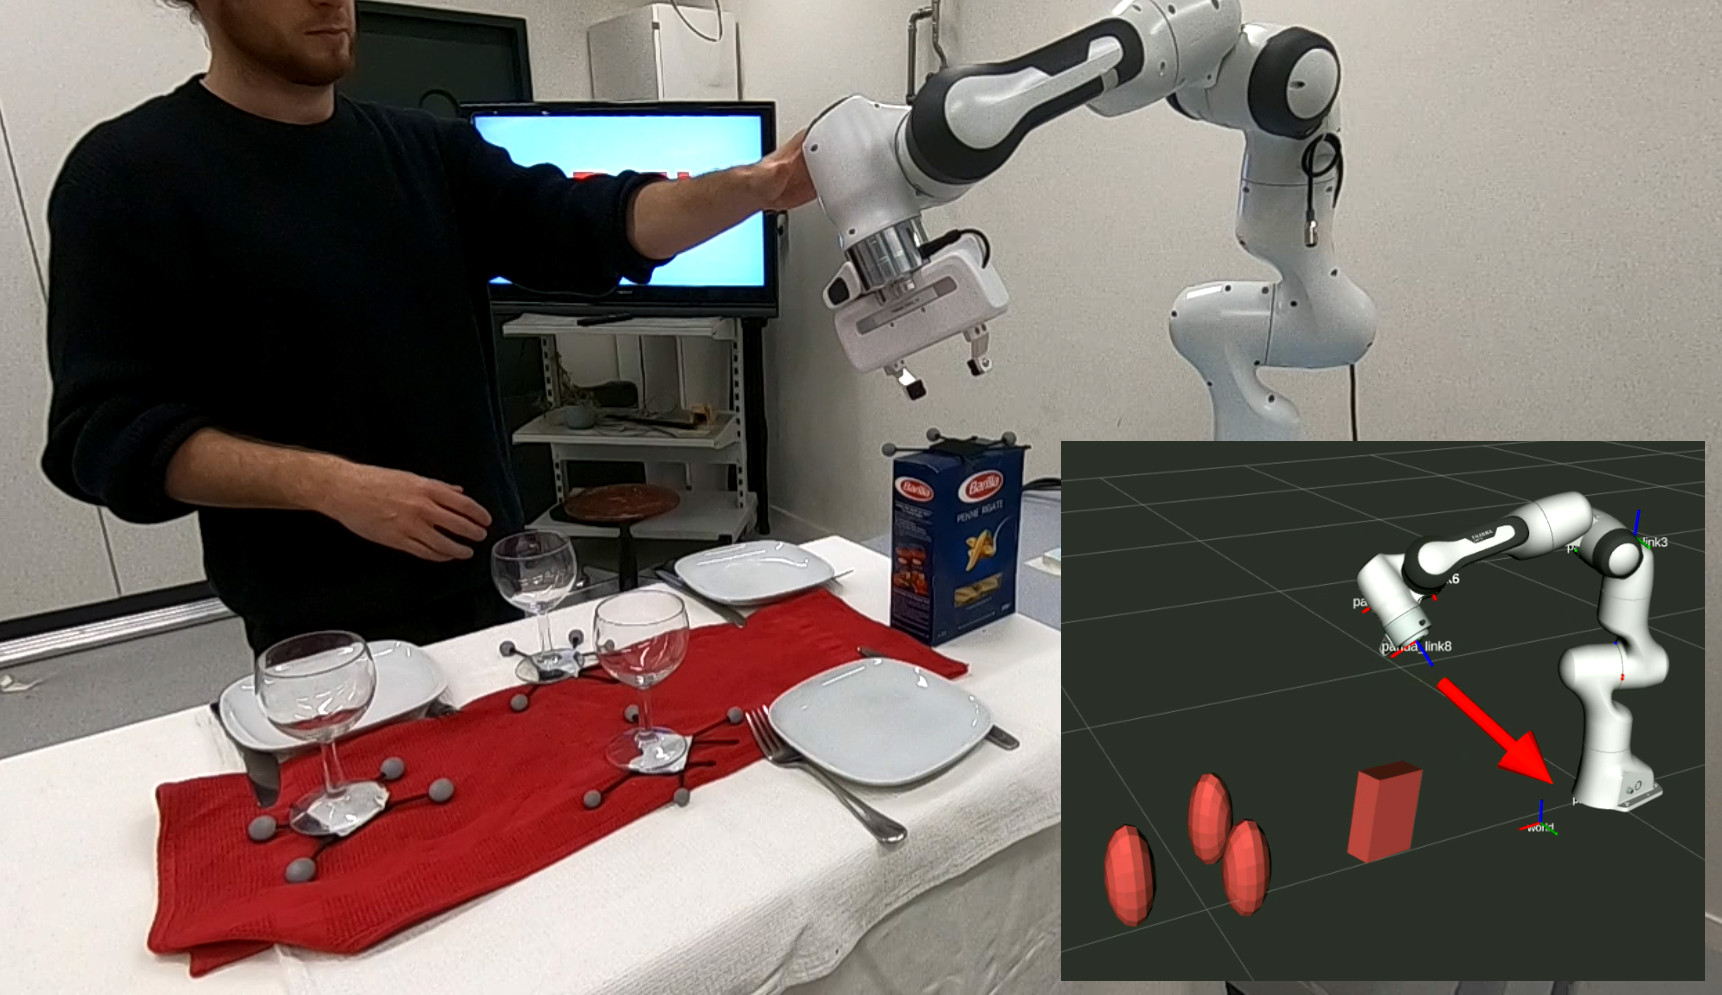
\includegraphics[width=0.5\textwidth]{figures/robot_arm_table_avoidance}}
\caption{
The proposed passive obstacle-aware controller lets the robot absorb external disturbances while ensuring collision avoidance. 
While tipping over the closed pasta box on this dinner table setup might be acceptable. Yet, the delicate wine glasses demand careful handling to prevent breakage.
}
\label{fig:table_avoidance_with_obstacle}
\end{figure}

This work incorporates dynamic obstacle avoidance using DS and variable impedance control, enhancing robotic movements' adaptability, reactivity, and safety. It allows the robot to navigate complex environments while proactively avoiding collisions and adeptly rejecting disturbances. We evaluate the performance of our approach through extensive simulations and practical implementation on a 7DoF robot arm, achieving robust and safe robot control in real-world scenarios.

\subsection{Related Work}

\subsubsection{Impedance Control}
Impedance control, a powerful feedback algorithm, effectively applies Cartesian impedance to nonlinear manipulators' end-points \parencite{takegaki1981new, hogan1985impedance}. The controller replaces the computationally intensive \textit{inverse kinematics} with the more straightforward \textit{forward kinematics}. Impedance control establishes a dynamic relationship between desired position, velocity, and force, offering a holistic control framework.
Initially, impedance controllers employed constant stiffness, but researchers have explored various dynamic control parameter approaches to enhance adaptability in complex environments \parencite{vanderborght2013variable, abu2020variable}. However, introducing dynamic parameters into the control framework requires taking special care of the system's stability.
Furthermore, admittance control is designed to adapt to external forces, while remaining stable contact \parencite{glosser1994implementation}. Admittance control can be interpreted as a special type of impedance control.

% Passivity with increased precision
Passive velocity controllers use a state-dependent velocity, which is converted into a control force through a damping control law. Since the controllers have variable damping parameters, stability can be guaranteed using storage tanks inspired by a virtual flywheel \parencite{li1999passive}. 
Furthermore, complex control parameters can be learned from human demonstrations. By continuously adapting the parameters, the controller can be observed to improve its tracking performance in direct human-robot collaboration tasks \parencite{gribovskaya2011motion}.
However, high compliance often results in decreased motion following. Yet, carefully designing the damping matrix, which increases stiffness in the direction of motion, but remains compliant otherwise, results in improved convergence \parencite{kronander2015passive}. 
Combining impedance controllers with admittance controllers can be used to increase accuracy in cooperative control
\parencite{fujiki2022series}.
However, these controllers' adaptations focus on improving movement accuracy rather than actively rejecting disturbances.

% Stable interaction controller
Impedance controllers play an important role in interaction tasks, as in these situations, the robot is subjected to forces that are hard to predict precisely. However, they must be actively managed to ensure stable contact without damage occurring. In these situations, passive controllers using storage tanks based on the system's energy allow to limit contact force \parencite{kishi2003passive}.
A general framework can be used to ensure that position-, torque-, and impedance controllers exhibit passivity during interaction tasks. This is achieved by interpreting the torque feedback as the shaping of the motor inertia. It allows the use of flexible robot arms for complex interaction tasks, such as insertion or wiping \parencite{albu2007unified}. 
By sensing the interaction force and actively adapting the trajectory based on the physical interaction force and the virtual repulsive force from the obstacle. This can be used for obstacle-aware motion generation \parencite{haddadin2010real}.
% Telemanipulation
Teleoperated systems of robot arms come with control delays and require a closed-loop controller of the robot that can adapt autonomously, ensuring stable and reliable performance. Passive controllers present themselves perfectly for such a task  \parencite{stramigioli2005sampled}. This method addresses the intricate dynamics of interactive systems, ensuring stable and reliable performance.
A similar approach involves slowly updating the desired position while incorporating a spring-damper model through an impedance controller, enabling seamless interaction with the teleoperated robotic system \parencite{lee2010passive}.
However, these models require human input for active collision avoidance.

% Energy tanks 
Many impedance controllers with time-varying control rely on energy tanks to ensure stability. This is a virtual state of the system, which is filled or emptied depending on the controller command. Limiting the energy tank to a maximum value ensures the system's stability  \parencite{ferraguti2013tank}. However, when this limit is reached, the controller is constrained and interferes with the controller's optimal functioning. This can result in the controller not achieving a main functionality, such as collision avoidance.
Alternatively, the impedance controller variables can be constrained by adapting the damping and stiffness, as well as their rate of change based on a Lyapunov function \cite{kronander2016stability}.

\subsubsection{Obstacle Avoidance}
% AFP / Obstacle avoidance / Motion Control
In dynamic environments, obstacle avoidance has to be quickly evaluated to ensure safe robot navigation. Repulsive force fields pointing away from obstacles can be used to create a collision-free motion \parencite{khatib1987unified}. 
However, these artificial potential fields are susceptible to local minima, which led to the introduction of navigation functions. A global function that combines the repulsive force fields while ensuring a global minimum and the goal \parencite{koditschek1990robot}. However, such functions depend on the distribution of the obstacles and are hard to adapt to dynamic environments and high dimensional spaces \parencite{loizou2022mobile}.


% \cite{brock2002task}, % Corresponding conference 
Passive controllers can also be used to track the desired motion of the artificial potential field while compensating for Coriolis and centrifugal forces \parencite{duindam2004passive}. 
Nonetheless, these methods lack the guarantee of disturbance repulsion around obstacles, which is addressed by the integration of circular fields, which rotates the robot's path around the obstacles \parencite{singh1996real}. 
This allows force-controlled navigation in cluttered environments, yielding convergence for simple obstacles \parencite{haddadin2011dynamic}. 
Conversely, repulsive fields can be combined with elastic, global planning \parencite{brock2002elastic} for improved convergence. This allowed adding a repulsive force from the obstacle, ensuring collision avoidance \parencite{tulbure2020closing}. 
However, methods based on artificial potential fields are prone to local minima in space around cluttered environments.

% Geometric Methods for Obstacle Avoidance / Force Control
Traditional tracking controllers often require complex linearization or simplification methods. However, a class of geometric tracking controllers enables exact control of nonlinear mechanical systems with low computational cost \parencite{udwadia2003new}. By reformulating control problems as a specific class of optimal controllers, this approach facilitates the derivation of standard control problems in robotics \parencite{peters2008unifying}. As a result, many geometric controllers directly output a control force, and hence do not rely on an additional (impedance) controller.
Integrating local Riemannian Motion Policies (RMP) has led to globally stable force-controlled motion \parencite{cheng2020rmp}. Moreover, advancements in position-dependent Riemannian metrics allow for improved task design using RMP and reactive force control under constraints \parencite{bylard2021composable}.
Geometric fabrics have emerged as a valuable mathematical tool for shaping a robot's nominal behavior while capturing essential constraints like obstacle avoidance, joint limits, and redundancy resolution \parencite{xie2020geometric}. Combining Finsler geometry and geometric fabrics has further enhanced path consistency \parencite{ratliff2021generalized}.
Integrating geometric fabric methods into classical mechanical systems has enabled various physical behaviors, notably exemplified in multi-obstacle avoidance for a 7DoF robot arm \parencite{van2022geometric}. Despite these significant achievements, the parametrization of geometric methods and their application to general systems remains challenging and hinders their wide acceptance.

% Dynamical system based avoidance + control
Harmonic potential functions can ensure the absence of local minima in free space \parencite{connolly1997harmonic}. In previous work, we combined harmonic potential functions with the dynamical system framework to obtain reactive, local minima-free motion \parencite{huber2019avoidance, huber2023avoidance}. It allows for generating a desired velocity based on the robot's position in real-time.
For implementation on a torque-controlled robot arm, we utilized a passive controller that closely adheres to the desired velocity \parencite{kronander2015passive}. However, one of the limitations of the passive controller is its inability to  account for the physical surroundings. This makes the robot susceptible to disturbances close to obstacles, potentially leading to collisions.

Although DS passive-controlled robots work well in interactive scenarios, they cannot ensure they navigate through an obstacle environment collision-free. For example, they often give in when being pushed toward an obstacle. This work presents a method to address this problem by modifying the passive control law design, making the controller aware of its environment.

\subsection{Contribution}
We introduce a passive controller that incorporates into the feedback control loop as visualized in Figure~\ref{fig:control_scheme_passive}. 
In this work, we make the following contributions:
\begin{itemize}
\item The design of the obstacle-aware passive controller
(Section~\ref{sec:obstacle_aware_passivity})
\item A passivity guarantee (without the need for a storage tank) which applies to general damping controllers (Theorem~\ref{theorem:passivity})
\item A collision avoidance analysis which provides insight into the path consistency around obstacles (Section~\ref{sec:collision_avoidance})
\item Discrete-time analysis to enable control parameter design which ensures stability (Section~\ref{sec:discrete_time_behavior})
\item Implementation and testing on 7DoF robot arm (Section~\ref{sec:evaluation})
\end{itemize}


\begin{figure}[thb]
  \center
  \includesvg[width=1.0\columnwidth]{figures/control_scheme_passive.svg}
\caption{The desired velocity $\vect f^b(\vecs \xi)$ can result from a learned velocity field or pointing towards a desired attractor $\vecs \xi^a$. The desired velocity is used to evaluate the obstacle avoidance velocity $\vect f(\vecs \xi)$, which is fed into the force controller to obtain the control force $\vect \tau_c$. In order to achieve collision avoidance, the distance function $\Gamma_o(\vecs \xi)$, the normal direction $\vect n_o(\vecs \xi)$, and the reference direction $\vect r_o(\vecs \xi)$ are evaluated for each obstacle $o = 1 .. N^\mathrm{{obs}}$.}
\label{fig:control_scheme_passive}
\end{figure}

% \section{Preliminaries}
Let $\vecs\xi \in \mathbb{R}^N$ describe the system's state in an $N \geq 2$ dimensional space, e.g., the robot's joint or Cartesian space positions.
The function $\vecs f(\vecs \xi): \mathbb{R}^N \rightarrow \mathbb{R}^N$ represents a smoothly defined dynamical system (DS) describing the desired velocity at a given state $\vecs \xi$.  
The first and second-order time derivatives are denoted by one and two dots over the symbol respectively, i.e., $\dot{\vecs \xi} =\frac{d}{dt} \vecs \xi$ is the systems velocity, and $\ddot{\vecs \xi} = \frac{d^2}{dt^2} \vecs \xi$ is the acceleration.
%Furthermore, all trajectories converge to the unique attractor state $\vecs \xi ^a \in \mathbb{R}^N$. 

\subsection{Obstacle Avoidance}
Let us assume the base velocity $\vect f^b(\vecs \xi): \mathbb{R}^N \rightarrow \mathbb{R}^N$, which describes the desired, state-dependent motion of the robot. 
As proposed by \cite{huber2019avoidance, huber2022avoiding}, an obstacle avoiding velocity $\vect f(\vecs \xi): \mathbb{R}^N \rightarrow \mathbb{R}^N$ can be achieved by a simple matrix multiplication (or modulation) as follows:
\begin{equation}
  \vecs f(\vecs \xi) = \textbf{E}(\vecs \xi) \text{diag} \left(\lambda^r, \lambda^e, ..., \lambda^e \right) \textbf{E}(\vecs{\xi})^{-1} \vect f^b(\vecs \xi)
  \label{eq:modulated} 
\end{equation}

The orthonormal basis matrix $\textbf{E} \in \mathbb{R}^{N \times N}$, defined as:
\begin{equation}
\textbf{E}(\vecs \xi) = \left[ \textbf{r}(\vecs \xi) \ \textbf{e}_1(\vecs \xi) \ ... \ \textbf{e}_{d-1}(\vecs \xi) \right]
\label{eq:matrix_E}
\end{equation}
where the tangent directions $\textbf{e}_{(\cdot)} \in \mathbb{R}^N$ are perpendicular to the surface normal $\vect n(\vecs \xi) \in \mathbb{R}^N$, see Fig.~\ref{fig:resultant_normal}. The reference vector $\textbf{r}(\vect{\xi}) =  \left( \vecs{\xi}-\vecs{\xi}^r \right) / \| \vecs \xi-\vecs \xi ^r \|$ is pointing towards the the reference point $\vecs \xi^r \in \mathbb{R}^N$. 
This construction of the basis matrix is valid for starshaped obstacles, i.e., shapes for which a reference point exists, from which a line in any direction only crosses the surface once \cite{huber2023avoidance}.

The  diagonal values $\lambda_{(\cdot)}$  in \eqref{eq:modulated} are often referred to as eigenvalues since they modify the length of the input velocity in specific directions. 
The eigenvalue in reference direction $\lambda^r(\vecs \xi) \leq 1$, is designed to reduce the velocity towards the obstacle, i.e., towards the reference point.  
Conversely, the velocity increases along the tangent direction using $\lambda^e(\vecs \xi) \geq 1$. This eigenvalues in reference direction $\lambda^r$ and tangent direction $\lambda^e$ are defined as:
\begin{equation}
\begin{split}
    \lambda^r(\vecs \xi) = 1 - 1 /\Gamma(\vecs \xi) , \quad \lambda^e(\vecs \xi) = 1 + 1 / \Gamma(\vecs \xi)
    \label{eq:eigenvalues}
    \end{split}
\end{equation}
with the continuous distance function $\Gamma(\vecs \xi) \in \mathbb{R}_{\geq 0}$, which has a value of $\Gamma(\vecs \xi) = 1$ on the boundary of an obstacle, and $\Gamma(\vecs \xi) > 1$ away from the surface (Fig.~\ref{fig:resultant_normal}). In this work, we use the following distance function
\begin{equation}
  \Gamma(\vecs \xi) = 1 + \| \vecs \xi - \vecs \xi^b \|  
  \quad \text{with} \quad
  \vecs \xi^b = b (\vecs \xi - \vecs \xi^r) + \vecs \xi^r
  \label{eq:distance_function}
\end{equation}
with $b \in \mathbb{R}_{>0}$, such that $\vect \xi^b \in \mathbb{R}^N$ lies on the surface of the obstacle.

\begin{figure}
\centerline{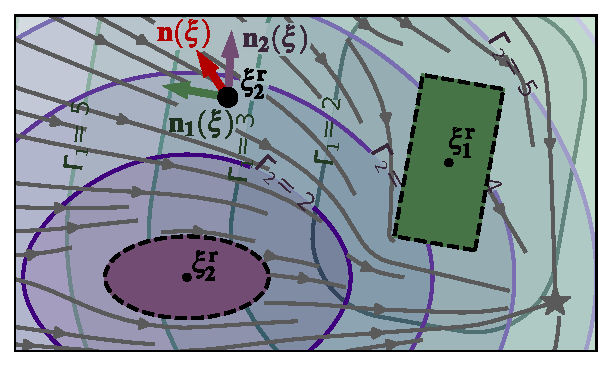
\includegraphics[width=0.5\textwidth]{figures/normal_and_gamma_field_visualization_annotated.pdf}}
\caption{
The $\Gamma$-field is defined individually for each of the obstacles. At each position $\vecs \xi$, we can evaluate the surface normal $\vect n(\vecs \xi)$. 
The velocity $\vect f(\vecs \xi)$ (gray) avoids collision with the obstacles and converges towards the attractor (star).}
\label{fig:resultant_normal}
\end{figure}

Modifying the base velocity $\vect f^b(\vecs \xi)$ with these eigenvalues values and \eqref{eq:modulated} leads to obstacle-avoiding dynamics $\vect f(\vecs \xi)$ which generate converging motion around starshaped obstacles.

\subsection{Force Control}

\subsubsection{Rigid Body Dynamics}
A force-controlled system is subject to acceleration effects, inertia, and external disturbances. Its general rigid-body dynamics based on the state $\vecs \xi$ are given as
\begin{equation}
\matd{M}(\vecs\xi)\vecs{\ddot\xi} + \matd{C}(\vecs\xi, \vecs{\dot\xi})\vecs{\dot\xi} + \vect g(\vecs\xi) = \vecs{\tau_c} + \vecs{\tau_e}
 \label{eq:robot_dynamics}
\end{equation}
where we have the mass matrix of the robot $\matd M(\vecs\xi) \in \mathbb{R}^{N \times N}$, the Coriolis matrix $\matd C(\vecs\xi,\vecs{\dot\xi}) \in \mathbb{R}^N$, the gravity vector $\vect g(\vecs\xi) \in \mathbb{R}^N)$, the control torque $\vecs{\tau_c} \in \mathbb{R}^N$, and the external torque, also referred as disturbance, $\vecs{\tau_e} \in \mathbb{R}^N$.

\subsubsection{Passive Control}
Passive interaction control \cite{kronander2015passive} offers a powerful method for computing control forces from a velocity field. This controller provides selective disturbance rejection based on the direction of the desired motion. Typically, the controller is configured with high damping along the direction of motion, ensuring rapid convergence of the robot's velocity to the desired value and achieving excellent tracking performance. In contrast, the controller exhibits high compliance in the direction perpendicular to the motion, enabling flexible behavior and greater resistance to external forces. The passive control force is evaluated as:
\begin{equation}
	\vecs{\tau_c} = \vect g (\vecs\xi) 
	% + \matd{D}(\vect \xi, \dot{\vect \xi}) \dot{\vect \xi}  
	+ \matd{D}(\vecs\xi) \left(\vecs f(\vecs\xi) - \vecs{\dot\xi} \right) 
\label{eq:control_command}
\end{equation}
This control law embeds a gravity compensation term $\vect g (\vecs\xi) \in \mathbb{R}^N$ and a positive-definite damping term, which dampens the difference between the desired velocity $\vecs f(\vecs\xi)$ and the actual velocity $\vecs{\dot\xi}$.

The positive definite damping matrix $\matd D(\vecs\xi) \in \mathbb{R}^{N \times N}$ is given as:
\begin{equation}
   \matd {D}(\vecs \xi) = \matd{Q}(\vecs\xi)\matd{S}(\vecs\xi) \matd{Q} (\vecs \xi)^{-1}
\label{eq:damping_matrix}
\end{equation}
where $\matd Q(\vecs \xi) = \left[ \vecs{q}_1 \, , \; \vecs q_2\ , \; ... \, , \; \vecs q_N \right] $ is an orthonormal basis matrix, of which the first vector is pointing in the desired direction of motion
\begin{equation}
    \vecs q_1(\vecs \xi) = \vecs q_1^f(\vecs \xi) = \dot{\vecs \xi} / \lVert \dot{\vecs \xi} \rVert \label{eq:velocity_unit_vector}
\end{equation}

The diagonal matrix $\matd{S}(\vecs\xi) \in \mathbb{R}^{N \times N}$ consists of damping factors $s_i \in \mathbb{R}_{>0}$ in the corresponding direction $i = 1 .. N$.
This design allows the separate design of the damping in the direction of motion and perpendicular to the motion.
Increased consistency with the desired velocity is achieved by setting the first damping factor to a relatively high value. Conversely, the damping in the remaining directions is set lower to allow compliance perpendicular to the motion, i.e., $s_i / s_1 \ll 1, \; i = 2 .. N$.

\subsection{Stability Analysis} \label{sec:trad_passive}
Considering varying control parameters carefully is crucial, as such a design can inject energy into a system, potentially leading to unstable behavior and damaging the system \cite{ferraguti2013tank}.
In human-robot interaction, the robot faces external disturbances of unknown nature. To achieve stable and bounded behavior in the face of such disturbances, \textit{passivity} analysis is a valuable tool. By employing passivity analysis, the control system can be designed to maintain stable responses (bounded system) in the presence of any external force (bounded input). 

\begin{definition}[Passivity \cite{willems1972dissipative, sepulchre2012constructive}] \label{def:passivity}
	A dynamical system with input $ u \in \mathcal{U}$ and output $y \in \mathcal{Y}$ is passive with respect to the supply rate $s : \mathcal{U} \times \mathcal{Y} \rightarrow{R}$ if, for any $u: \mathbb{R}_{>0} \rightarrow \mathcal{U}$ and any time $t^* \geq 0$ the following is satisfied
  \begin{equation}
	  \int_0^{t^*} s \left( u(t),  y (t) \right) d \tau \geq S(t^*) - S(0) 
  \end{equation}
  where $S(t) \in \mathbb{R}_{\geq 0}$ is the storage function.
\end{definition}

The feedback loop combining two passive systems results in a passive system \cite{sepulchre2012constructive}. Hence, if the controller is passive, its application to a (passive) environment-hardware system results in a passive system.

\subsection{Contribution}
We introduce a passive controller that incorporates into the feedback control loop as visualized in Figure~\ref{fig:control_scheme_passive}. 
In this work, we make the following contributions:
\begin{itemize}
\item The design of the obstacle-aware passive controller
(Section~\ref{sec:obstacle_aware_passivity})
\item A passivity guarantee (without the need for a storage tank) which applies to general damping controllers (Theorem~\ref{theorem:passivity})
\item A collision avoidance analysis which provides insight into the path consistency around obstacles (Section~\ref{sec:collision_avoidance})
\item Discrete-time analysis to enable control parameter design which ensures stability (Section~\ref{sec:discrete_time_behavior})
\item Implementation and testing on 7DoF robot arm (Section~\ref{sec:evaluation})
\end{itemize}

\ifthesis
\,
\else
\begin{figure}[thb]
  \center
  \includesvg[width=1.0\columnwidth]{figures/control_scheme_passive.svg}
\caption{The desired velocity $\vect f^b(\vecs \xi)$ can result from a learned velocity field or pointing towards a desired attractor $\vecs \xi^a$. The desired velocity is used to evaluate the obstacle avoidance velocity $\vect f(\vecs \xi)$, fed into the force controller to obtain the control force $\vect \tau_c$. In order to achieve collision avoidance, the distance function $\Gamma_o(\vecs \xi)$, the normal direction $\vect n_o(\vecs \xi)$, and the reference direction $\vect r_o(\vecs \xi)$ are evaluated for each obstacle $o = 1 .. N^\mathrm{{obs}}$.}
\label{fig:control_scheme_passive}
\end{figure}
\fi

\subsection{Problem Statement}
Following assumptions are made about the desired velocity $\vecs f(\vecs\xi)$:
\begin{enumerate}
    \item $\vecs f(\vecs\xi)$ is continuously  for all reachable states.
    %% \item $\vecs f(\vecs\xi)$ has a single equilibrium point $\vecs\xi^a$, such that $\{ \vecs \xi : \vecs f(\vecs \xi) = \vecs 0 \} = \{ \vecs\xi^a \}$. 
    \item $\vecs f(\vecs\xi)$ is bounded, i.e., there exists a constant $v^{\mathrm{max}} \in \mathbb{R}$ such that $\| \vecs f(\vecs\xi) \| \leq v^{\mathrm{max}} \;\; \forall \, \vecs \xi \in \mathbb{R}^N$
    \item It leads to a collision-free motion $\vecs{n_o}(\vecs\xi)^T \vecs f(\vecs\xi) \geq 0$ as $\Gamma_o \rightarrow 1 
  \quad \forall o = 1 .. N^{\mathrm{obs}}$
  with the normal $\vecs n_o (\vecs \xi)$ and distance $d_o$ of the $o$-th obstacle. 
\end{enumerate}

Note that velocities obtained using DSM, given in \eqref{eq:modulated}, fulfill these conditions if velocity function $\vecs f^I$ is continuous and bounded.


% \subsection{Nomenclature}
Note, that in this Chapter, the desired velocity $\vect f: \mathbb{R}^N \rightarrow \mathbb{R}^N$ is expected to be avoiding collisions, and, as such, might be obtained from a vector-field-based collision avoidance algorithm as described in the previous chapters. 

Moreover, the velocity $\dot{\vecs \xi} \mathbb{R}^N$ describes the actual velocity of the system, specifically the robot agent, and $\ddot{\vecs \xi} \mathbb{R}^N $ is the acceleration.

\section{Obstacle-Aware Passivity} \label{sec:obstacle_aware_passivity}
We propose a novel controller, which ensures passivity as defined in \eqref{eq:control_command} but adapts the damping matrix given in \eqref{eq:damping_matrix} based on the desired velocity $\dot{\vecs \xi}$ and obstacles in the surrounding. 
Far away from obstacles, the system is designed to follow the initial velocity, but approaching the obstacle increases the damping, decreasing the chance of a collision.

\ifthesis
\begin{figure}
\centerline{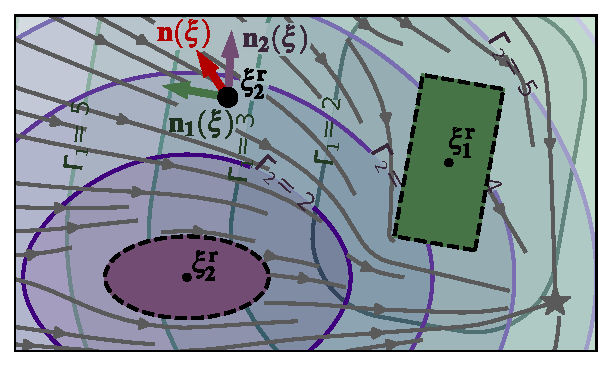
\includegraphics[width=0.7\columnwidth]{figures/normal_and_gamma_field_visualization_annotated.pdf}}
\caption{
The $\Gamma$-field is defined individually for each of the obstacles. At each position $\vecs \xi$, we can evaluate the surface normal $\vect n(\vecs \xi)$. 
The velocity $\vect f(\vecs \xi)$ (gray) avoids collision with the obstacles and converges towards the attractor (star).}
\label{fig:resultant_normal}
\end{figure}
\fi


Hence, the damping matrix $\matd D(\vecs\xi) \in \mathbb{R}^{N \times N}$ smoothly changes from being aligned with the direction of the velocity, as used in \parencite{kronander2015passive}, to be aligned with the averaged normal of the obstacles. The desired damping matrix transitions between velocity preserving and collision avoidance using a smoothly defined linear combination:
\editcolor{
\begin{equation}
	\matd D(\vecs\xi, \dot{\vecs \xi}) = \left(1 - w(\vecs\xi) \right) {\matd D^{f}}(\vecs\xi) + w(\vecs\xi)  {\matd D^{\mathrm{o}}}(\vecs\xi, \dot{\vecs \xi}) \label{eq:damping_summation}
\end{equation}
}
The damping matrix is made up of two components: the velocity damping. $\matd D^f \in \mathbb{R}^{N \times N}$ which prioritizes following the desired velocity similar to \parencite{kronander2015passive}, and the obstacle damping $\matd D^{\mathrm{o}} \in \mathbb{R}^{N \times N}$ which is designed to reject disturbances towards obstacles. The two damping matrices are positive definite and are smoothly summed using the danger weight $w(\vecs\xi) \in [0, 1]$. Far away from obstacles the weight reaches $w(\vecs \xi) = 0$, whereas $w(\vecs \xi) = 1$ when approaching a boundary:
\begin{equation}
  \begin{split}
w(\vecs\xi) =
\max \left(0,  \frac{\Gamma^{\mathrm{crit}} - \Gamma(\vecs\xi)}{\Gamma^{\mathrm{crit}} - 1} \right) \| \vecs n(\vecs \xi) \| \\
\text{with} \quad
\Gamma(\vecs\xi) = \min_{o = 1, ..., N^{\mathrm{obs}}} \Gamma_o(\vecs\xi)
\end{split}
\label{eq:weight_function}
\end{equation}
The critical distance \iflong $\Gamma^{\mathrm{crit}} \in \mathbb{R}_{>0}$ \fi defines the distance where the system increases the damping towards the obstacle.
${\matd D^f}(\vecs\xi)$ and $\matd {D^{\mathrm{obs}}}(\vecs\xi)$ follow design given in \eqref{eq:damping_matrix} and are positive definite matrices, thus $\matd {D}(\vecs\xi)$ is positive definite, too.

\iflong
\begin{figure}
  \center
  % \includesvg[width=0.7\columnwidth]{figures/damping_basis_construction.svg}
  \ifthesis
  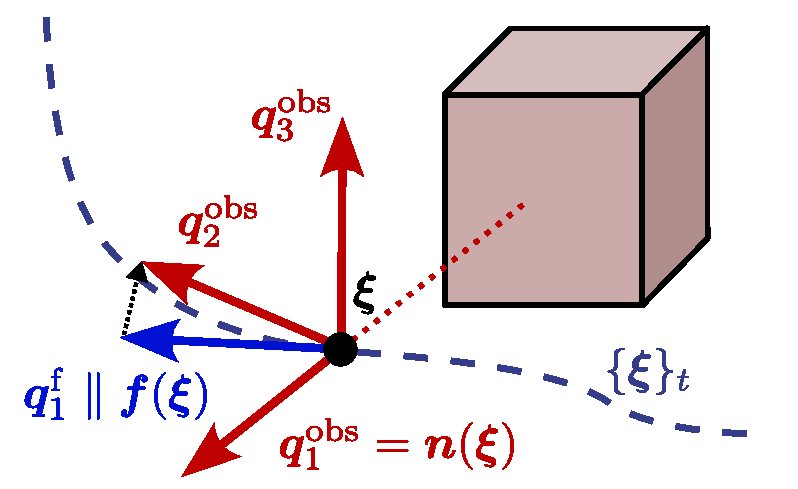
\includegraphics[width=0.5\columnwidth]{figures/damping_basis_construction.pdf}
  \else
  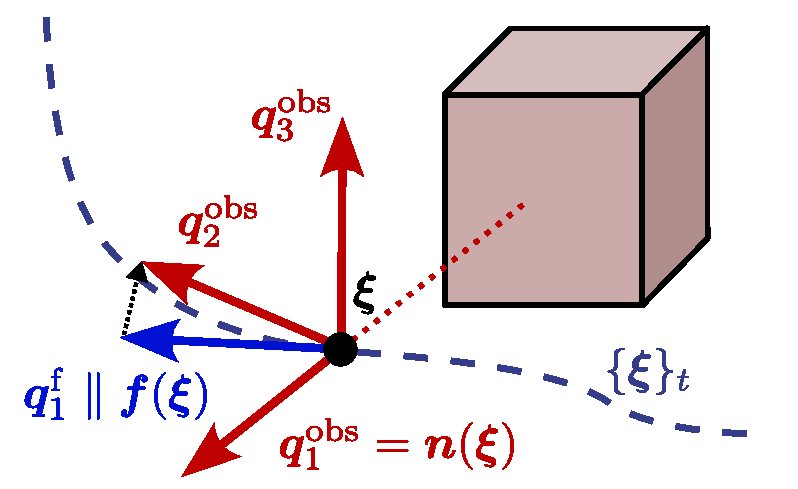
\includegraphics[width=1\columnwidth]{figures/damping_basis_construction.pdf}
  \fi
\caption{The damping matrix enforcing desired velocity following $\matd{D}^{f}$ has the first basis vector $\vect q_1^{f}$ which points along the avoidance velocity $\vect f(\vecs \xi)$. The damping matrix to enforce collision avoidance $\matd{D}^{\mathrm{obs}}$ uses the normal $\vect n(\vecs \xi)$ to construct the first direction of the decomposition basis $\vect q^{\mathrm{obs}}_1$.}
\label{fig:damping_basis_construction}
\end{figure}
\fi

\subsection{Damping for Collision Repulsion} \label{sec:obstacle_repulsion}

\subsubsection{Normal Direction}
The damping matrix $\matd D^{\mathrm{o}}(\vecs \xi)$ rejects velocities in the direction of the obstacles. To allow this, we introduce an averaged normal direction:
\begin{equation}
  \vecs n(\vecs\xi) = \sum_{o=1}^{N^{\mathrm{o}}} \vecs{n_o}(\vecs\xi)
  \frac{1 / (\Gamma_o(\vecs \xi) - 1)}{\sum_{p=1}^{N^\mathrm{o}} 1 / (\Gamma_p(\vecs \xi) - 1)}
  \label{eq:averaged_normal}
\end{equation}
 where the unit normals $\vecs{n_o} (\vecs\xi)$ pointing away from the obstacle $o = 1,  ..,  N^{\mathrm{o}}$ and are perpendicular to the surface, see Figure~\ref{fig:resultant_normal}. 

The averaged normal $\vecs n(\vecs \xi)$ is a weighted linear combination of the obstacles' normals, giving more importance to closer obstacles.
Additionally, the averaged normal converges to an obstacle normal as we converge towards it, i.e., $\lim_{\Gamma_o(\vecs \xi) \rightarrow 1} \vecs n(\vecs \xi) = \vecs n_o(\vecs \xi)$.
Note that the averaged normal is a zero-vector when two obstacles oppose each other. 

\subsubsection{Decomposition Matrix}
The decomposition matrix $\matd Q^{\mathrm{o}}(\vecs \xi)$ has its first vector aligned with the normal to the obstacle: 
\begin{equation}
    \vecs q_1^{\mathrm{o}}(\vecs\xi) =  \vecs n(\vecs\xi) / \lVert\vecs n(\vecs\xi)\rVert 
    \quad \forall \, \vecs \xi : \lVert\vecs n(\vecs\xi)\rVert  > 0
    \label{eq:first_obstacle_basis}
\end{equation}

In the case that $\lVert\vecs n(\vecs\xi)\rVert = 0$, the danger weight $w(\vecs \xi)$ from \eqref{eq:weight_function} reaches 0. Hence, the obstacle-aware damping in \eqref{eq:damping_summation} has no effect and is not evaluated.


The second vector is set to be aligned with the desired velocity as much as possible, allowing increased velocity following \iflong (Fig.~\ref{fig:damping_basis_construction}) \else (Fig.~\ref{fig:resultant_normal})\fi. However, it has to remain orthonormal to $\vect q_1^{\mathrm{o}}$
\begin{equation}
  \vecs q_2^{\mathrm{o}} = \frac{\hat{\vecs q}_2^{\mathrm{o}}}{\| \hat{\vecs q}_2^{\mathrm{o}} \|}
  \quad
  \hat{\vecs q}_2^{\mathrm{o}} = \vecs q_1^{f} - \vecs q_1^{\mathrm{o}} p \quad  \forall \, \vecs \xi : | p | < 1
\end{equation}
where velocity unit vector $\vecs q_1^{f}$ is defined in \eqref{eq:velocity_unit_vector}, and the object weight is evaluated as $p = \dotprod{\vecs q_1^{\mathrm{o}}}{\vecs q_1^{f}}$. 
For the case that $| p | = 1$, the second basis $\vecs q_2^{\mathrm{o}}$ is set to be any orthonormal vector. The remaining vectors $\vecs q_d^{\mathrm{o}}, d = 3, ..., N$ are constructed to form an orthonormal basis to the first two.

\subsubsection{Damping Values}
We define the values of the diagonal matrix $\matd{S}^{\mathrm{o}}(\vecs \xi)$ as\begin{equation}
  \matd{S}_d^{\mathrm{o}}(\vecs \xi) =
  \begin{cases}
    s^{\mathrm{o}} & d = 1 \\
    | p | s^c + (1 - | p |) s^{f} & d = 2 \\
    s^c & d = 3, ..., N
  \end{cases}
  \label{eq:obstacle_damping_values}
\end{equation}
where the damping along the nominal direction $s^{f} \in \mathbb{R}_{>0}$, obstacle-damping $s^{\mathrm{o}} \in \mathbb{R}_{>0}$, and the compliant-damping $s^c \in \mathbb{R}_{>0}$ are user-defined parameters which determine the behavior of the passive-controller. The first entry of $\matr{S}^{\mathrm{o}}$ dictates the damping towards the obstacle, and the second entry the desired velocity following. Note how the second value approaches the compliant damping, as normal and velocity become parallel.

To ensure continuity across time of the control force as defined in \eqref{eq:control_command}, the values of the diagonal damping matrix  $\matd{S}^{\mathrm{o}}(\vecs \xi)$ in the tangent directions are equal when the normal aligns with the velocity:
\begin{equation}
    \lim_{| p | \rightarrow 1} \matd{S}_d = \matd{S}_e, 
    \quad d > 2, ..., N, \, e > 2, ..., N
\end{equation}
Hence, the choice of orthonormal vectors $\vecs q_d^{\mathrm{o}}, d > 2, ..., N$ does not influence the control force as long as the matrix $Q^{\mathrm{d}}$ has full rank.


\subsubsection{Damping Only Towards Obstacle} \label{sec:damping_only_toward}
In the presence of an obstacle, the disturbances should be damped strongly when the agent is pushed against the obstacle. Conversely, the system can remain compliant if the motion is away from the obstacle. This is achieved by setting updating the first damping value $\matd{S}^{\mathrm{o}}_1$ if the robot is moving away from the surface: 
\editcolor{
\begin{equation}
	\matd{S}_1^{\mathrm{o}} (\vecs \xi, \dot{\vecs \xi}) =
  \begin{cases}
    s^{\mathrm{o}} & \text{if} \;\; \left(\vect f(\vecs \xi) - \vecs{\dot \xi} \right)^T \vecs n(\vect \xi) > 0 \\
    s^{\mathrm{c}} & \text{otherwise}
  \end{cases}
  \label{eq:leaving_compliance}
\end{equation}
}

Since $\vect q_1^o(\vecs \xi)$ given in \eqref{eq:first_obstacle_basis} is pointing along the obstacle normal $\vect n(\vecs \xi)$, the first obstacle damping value $\matd{S}_1^{\mathrm{o}} (\vecs \xi)$ does not have any effect on the control force $\vect \tau^c$ given in \eqref{eq:control_command} when $\left(\vect f(\vecs \xi) -  \vecs{\dot \xi} \right)^T \vecs n(\vect \xi) = 0$.
Hence, the damping value can be discontinuous across time, but the resulting control force remains continuous.


\subsection{Damping for Velocity Preservation}
The decomposition matrix $\matd{Q}^{f}$ is an orthonormal basis with the first vector being parallel to the desired velocity $\vect f(\vecs\xi)$\iflong, as proposed in Section~\ref{sec:trad_passive}\fi. Hence, the values of the diagonal matrix $\matd S^{f}$ are high in the direction of the desired velocity (first component) but more compliant in the remaining directions. 
Moreover, the damping is set to ensure that when passing a narrow passage between two obstacles, where the normal vector cancels $\vect n(\vecs \xi) \approx \vect 0$, with additionally a low distance value $\Gamma(\vecs \xi) \approx 1$, the damping perpendicular to the velocity direction is high. We set:
\begin{equation}
  \begin{split}
  & \matd{S}^{f}_{d} =
  w^p s^{\mathrm{o}} + 
  \begin{cases}
   (1- w^p) s^f & d = 1 \\
    % w^p s^{\mathrm{o}} + (1- w^p) s^s & d = 2 .. N 
   (1- w^p) s^s & d = 2, ..., N 
  \end{cases} \\
  & \text{with} \quad
  %w^p = \min \left(1,  \| \vecs n(\vecs \xi) \|^2 + \left(\frac{\Gamma(\vecs \xi) -1}{\Gamma^{\mathrm{crit}} - 1}\right) ^2 \right)
   w^p = \min \left(1,  \| \vecs n(\vecs \xi) \|^2 +  \Delta \Gamma ^2 \right) \\
   & \text{and} \quad \Delta \Gamma = \max \left(\frac{\Gamma^{\mathrm{crit}} -\Gamma(\vecs \xi)}{\Gamma^{\mathrm{crit}} - 1}, 0\right)
  \end{split}
  \label{eq:velocity_damping}
\end{equation}

\subsection{Cluttered Environments}
In a cluttered environment, the normal vectors of the individual obstacles can be opposing. And hence using \eqref{eq:averaged_normal} and \eqref{eq:weight_function}, we get: 
\begin{equation}
    \| \vecs n(\vecs \xi) \| \rightarrow 0
    \quad \text{and} \quad
    \lim_{\Gamma (\vecs \xi) \rightarrow 1} w (\vecs \xi) = 0
\end{equation}
Additionally using \eqref{eq:damping_summation} and \eqref{eq:velocity_damping} we obtain:
\begin{equation}
    \lim_{\Gamma \rightarrow 1, \| n \| \rightarrow 0} \matd{D}(\vecs \xi) 
    = \matd{D}^S(\vecs \xi) + 0 
    =  \matd{I} s^o
\end{equation}

Hence, there is high damping in all directions to reject disturbances towards potential obstacles and ensure a collision-free motion even in cluttered environments.

\iflong
\subsection{Damping Parameter Design}
Higher values for the damping parameters $s^{(\cdot)}$ generally result in improved velocity following and disturbance repulsion, whereas lower values allow more compliant behavior.
The damping value in the direction of the obstacle is set high $s^{\mathrm{o}}$ to ensure obstacle avoidance even in the presence of high disturbances. 
Conversely, the damping in the direction of the velocity $s^{f}$ is set medium to high, as the system should follow the desired velocity $\vect f(\vecs \xi)$. However, it should remain compliant if needed.
Finally, to facilitate interaction, a low damping value $s^{c}$ should be chosen for all other directions.
This can be summarized as:
\begin{equation}
s^{\mathrm{o}} \geq s^{f} \gg s^{c} > 0
\end{equation}
\fi

\subsection{Passivity Analysis}
The stability analysis of the system gives information about the region of stability of the proposed controller. We analyze passivity by observing the evolution of the kinetic energy of the system, given as:
\begin{equation}
	W(\vecs \xi, \vecs{\dot \xi}) = \frac{1}{2}  \dot{\vecs{\xi}}^T \matd{M}(\vecs \xi) \dot{\vecs{\xi}} \label{eq:energy_system}
\end{equation}

\begin{lemma} \label{lemma:passivity}
  % Let $\vect f(\vecs \xi)$ be the desired velocity with bounded magnitude, i.e., $\| \vect f(\xi) \| < \infty, \forall \xi \in \mathbb{R}^N$.
   Let us assume a robotic system as described in \eqref{eq:robot_dynamics} is controlled using \eqref{eq:control_command} using the damping matrix $\matd D(\vecs \xi)$ given in \eqref{eq:damping_summation} with damping values $s_d = 1, d = 1 .. N$.
   The system is passive with respect to the input-output pair $\vecs \xi_e$, $\vecs{\dot \xi}$ when exceeding the desired velocity $\vect f(\vecs \xi)$ , i.e., $\dot{W} \leq \vecs{\dot \xi}^T \vecs \tau^e, \; \forall \vecs \xi \in \mathbb{R}^N: \| \vecs{\dot \xi} \| \geq \| \vect f(\vecs \xi) \|$ and the storage function being the kinetic energy $W \in \mathbb{R}_{>0}$ given in \eqref{eq:energy_system}
\end{lemma}

\begin{proof}
The time derivative of storage function $W$ can be evaluated as:
\begin{align}
  % \begin{split}
	& \dot W(\vecs \xi, \vecs{\dot \xi}) =
    \vecs{\dot \xi}^T \matd M(\vecs \xi) \vecs{\ddot \xi}  + \frac{1}{2} \vecs{\dot \xi}^T \dot{\matd M}(\vecs \xi) \vecs{\dot \xi}  \nonumber \\
  &= \frac{1}{2} \vecs{\dot \xi}^T \left( \dot{\matd M}(\vecs \xi) - 2 \matd C(\vecs \xi) \right) \dot{\vecs \xi} - \vecs{\dot \xi}^T \matd{D}(\vecs \xi) \left(\vecs{\dot \xi} - \vect f(\vecs \xi) \right) + \vecs{\dot \xi}^T \vecs \tau^e \nonumber \\
  &= - \vecs{\dot \xi}^T \matd{D}(\vecs \xi) \left( \vecs{\dot\xi} - \mathbf{f}(\vecs \xi) \right) + \vecs{\dot\xi}^T \vecs{\tau}^e
  % \end{split}
\end{align}
where the second order dynamics $\vecs{\ddot \xi}$ are evaluated according to the rigid body dynamics defined in \eqref{eq:robot_dynamics}. Furthermore, $\dot{\matd M} - 2 \matd C$ is skew-symmetric for any physical system; hence, the corresponding summand is zero.

% \subsubsection{Stability with Uniform Damping}
Let us investigate the region where the passivity holds. Since in the Lemma, we assumed all damping values being equal to one, we have:
\begin{equation}
	\matd{D}({\vecs \xi}) = \matd{Q}({\vecs \xi}) \matd{S} ({\vecs \xi}) \matd{Q}({\vecs \xi})^{-1}= \matd{Q}({\vecs \xi}) \matd{I} \matd{Q}({\vecs \xi})^{-1} = \matd{I}
\end{equation}
where $\matd{I} \in \mathbb{R}^{N \times N}$ is the identity matrix.

It follows that the system is passive with respect to the input, the external force $\tau^e$, and the output, the velocity $\dot {\vecs \xi}$, as long as:
\begin{equation}
	\dot{\boldsymbol {\vecs \xi}}^T \matd{D}({\vecs \xi}) \left(\dot{\boldsymbol {\vecs \xi}} - \boldsymbol{f}(\boldsymbol {\vecs \xi}) \right) = 
    \dot{{\vecs \xi}} ^ T \Delta \vect{f}  \geq 0 
 \; , \quad
 \Delta \vect{f} = \dot{{\vecs \xi}} - \vect{f}({\vecs \xi})
 \label{eq:passivity_condition}
\end{equation}

On the border of this region, the two vectors $\Delta \vect{f}$ and $\dot{{\vecs \xi}}$ are orthogonal.
Hence, using Thale's theorem, this region can be interpreted as a circle in velocity-space with radius $\| \vect{f} ({\vecs \xi}) \| / 2$ and center $\vect{f}({\vecs \xi}) / 2$, see Figure~\ref{fig:passivity_analysis}.

\begin{figure}[thb]
	\centering
	% \includesvg[width=0.7\columnwidth]{figures/passivity_analysis.svg}
	\ifthesis
    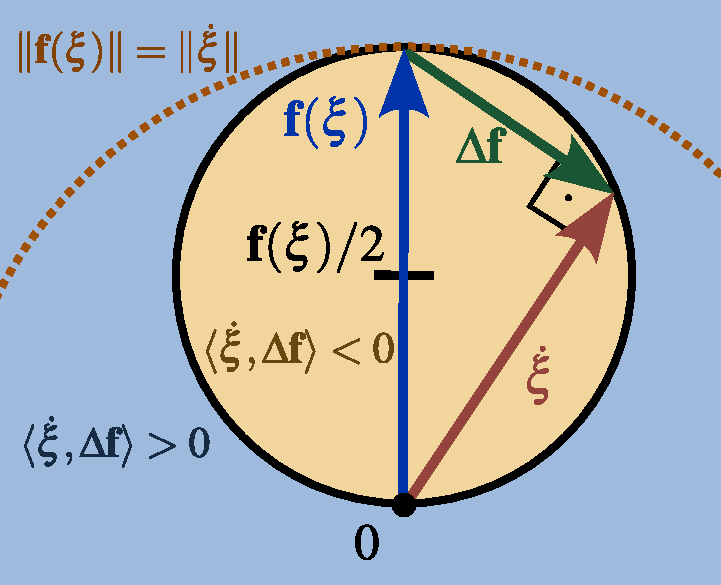
\includegraphics[width=0.7\columnwidth]{figures/passivity_analysis}
	\else
    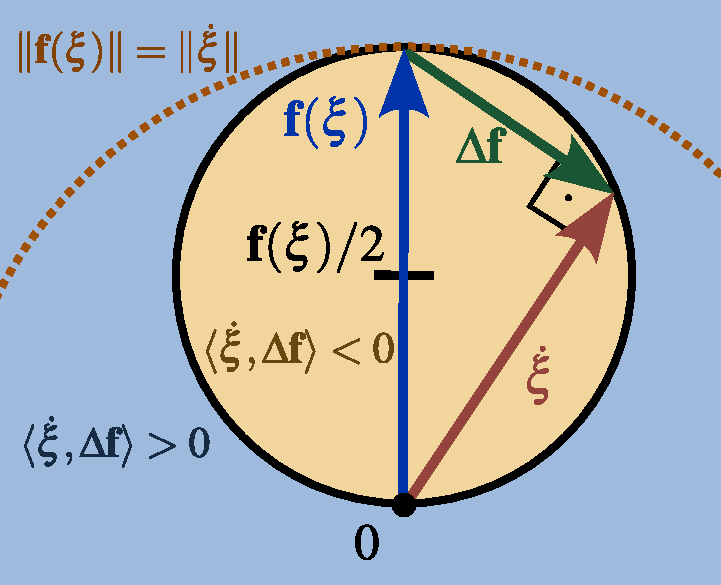
\includegraphics[width=.7\columnwidth]{figures/passivity_analysis}
	\fi
	\caption{Analyzing the system in velocity-space, yields that the system is passive if it has a velocity $\dot{\vecs \xi}$ larger than the desired velocity $\vect f(\vecs \xi)$, i.e., outside the dashed circle.
    However, the system can be non-passive for small velocities when  $\dotprod{\dot{\vecs \xi}}{\Delta \vect f} < 0$ (yellow circle).}
	\label{fig:passivity_analysis}
\end{figure}

Moreover, the system is passive as long as the observed velocity $\dot{{\vecs \xi}}$ is outside the circular-red region, which is a subset of the region where the magnitude of the observed velocity is smaller than the desired velocity $\vect {f}({\vecs \xi})$, i.e.,
\begin{equation}
	\dot W({\vecs \xi}, \dot{{\vecs \xi}}) \leq \dot{{\vecs \xi}}^T \vecs \tau^e
 \quad \forall {\vecs \xi} : \| \dot{{\vecs \xi}} \| \geq\| \vect{f}({\vecs \xi}) \| 
\end{equation}

\end{proof}

As in the orange region, the system is not passive; the storage function $W$ could increase, and hence, the velocity $\dot {\vecs \xi}$ increases non-passively. This behavior is not unexpected, as the controller is designed to approach the desired dynamics $\vect{f}({\vecs \xi})$. Hence, as long as the desired velocity is not reached, the kinetic energy increases even with no force input $\vecs \tau^e$. However, as soon as the system velocity $\dot{\vecs \xi}$ exceeds the desired velocity $\vect f(\vecs \xi)$, the system behaves passively. We can use this to ensure the stability of the system:

\begin{theorem}  \label{theorem:passivity}
  Let $\vect f(\vecs \xi)$ is the desired velocity with bounded magnitude, i.e., $\| \vect f(\vecs \xi) \| < v^{\mathrm{max}}, \forall \vecs \xi \in \mathbb{R}^N$.
   The closed loop system \eqref{eq:robot_dynamics} using the controller from \eqref{eq:control_command} and the damping matrix $\matd D(\vecs \xi)$ given in \eqref{eq:damping_summation} is bounded-input, bounded-output (BIBO) stable with respect to the input disturbance force $\vect \tau^e$, and output the velocity $\dot{\vecs \xi}$ for all times $T = 0, \, .., \, \infty$.
\end{theorem}
 
\begin{proof}
% From Lemma~\ref{lemma:passivity}, the system is passive when the magnitude of the velocity is larger than the dynamics, i.e. $\| \dot{\vecs \xi} \| > \|\vect f(\vecs \xi) \|$, the orange circle in Figure~\ref{fig:passivity_analysis}.
% The system is not passive inside this region, and the velocity $\dot {\vecs \xi}$ can increase. However, the velocity increase is limited to staying below $\| \vect f({\vecs \xi}) \|$ before the system enters the region where it is passive. Hence, the control cannot introduce unexpected energy.
% It follows that the system has a bounded output as long as the desired velocity $\vecs{f}({\vecs \xi})$ is stable and the input $\int_{0}^T \dot{{\vecs \xi}}^T \vecs \tau^e dt$ is bounded. 

To ensure BIBO stability, let us analyze the integral of the impulse of the response for the external force $\vecs \tau^e$: 
\begin{equation}
	\begin{split}
	  \int_{0}^{T} \left\| \dot{\vecs \xi} \right\| \; dt 
	  & = \int_{t \notin \mathcal{T}_n} \left\| \dot {\vecs \xi} \right\|  \, dt + \int_{t \in  \mathcal{T}_n} \left\| \dot {\vecs \xi} \right\| \;  dt \\ 
	  % & = \int_{t : \| \dot{\vecs \xi} \| > \| \vect f(\vecs \xi) \|} \dot {\vecs \xi} \, dt + \int_{t : \| \dot{\vecs \xi} \| \leq \| \vect f(\vecs \xi) \|} \dot {\vecs \xi} \;  dt \\ 
	  % & \leq \int_{t \notin \mathcal{T}_n} \left| \dot {\vecs \xi} \right| dt + v^{\mathrm{max}}  T_n \\ 
	  & \leq K_p + v^{\mathrm{max}} T_n
\end{split}
\label{eq:bibo_velocity}
\end{equation}
where $\mathcal{T}_n$ denotes the set of time instances where the system is not shown to be passive (Fig.~\ref{fig:passivity_analysis}), specifically $\| \dot{\vecs \xi} \| \leq \| \vecs f (\vecs \xi) \|$, and $T_n \in \mathbb{R}_{\geq 0}$ is the total duration which the system spends in this region. Additionally, from passivity in the inner region, the system is bounded by a constant $K_p \in \mathbb{R}_{\geq 0}$.
Hence, the impulse response is bounded, and the system is BIBO stable.

% \subsubsection{Stability with General Damping}
However, from \eqref{eq:damping_summation}, we know that a general damping matrix $\matd{S}(\vecs \xi)$ can have non-uniform diagonal values. This is analyzed by introducing the coordinate transfers:
\begin{equation}
	\vecs{\bar{v}} = \sqrt{\matd{S}({\vecs \xi})} \matd{Q}({\vecs \xi})^{-1} \dot{{\vecs \xi}}
	\;\; \text{and} \;\;
	\bar{\Delta \vect f} = \sqrt{\matd{S}({\vecs \xi})} \matd{Q}({\vecs \xi})^{-1} \Delta \vect{f}
\end{equation}
where the square root of the diagonal matrix $\matd{S}({\vecs \xi})$ is taken element-wise.

The transfer is then used to rewrite \eqref{eq:passivity_condition} as:
\begin{equation}
\dot{\vecs \xi}^T \matd{D}({\vecs \xi}) \Delta \vect{f} = \vecs{\dot \xi}^T \matd{Q}({\vecs \xi}) \matd{S}({\vecs \xi}) \matd{Q}({\vecs \xi})^{-1} \Delta \vect{f} = \vecs{\bar v}^T \bar{\Delta \vect f}
\end{equation}

Hence, the BIBO analysis of \eqref{eq:bibo_velocity} applied to the transformed system results as:
\begin{equation}
\begin{split}
	  & \int_{0}^{T} \left\| \vecs{\bar v} \right\| \; dt   
	   = \int_{t \notin \bar{\mathcal{T}}_n} \left\| \vecs{\bar v} \right\|  \, dt + \int_{t \in  \bar{\mathcal{T}}_n} \left\| \vecs{\bar v} \right\| \;  dt  \\ 
   & < K_p + v^{\mathrm{max}} \bar T_n 
   {\max{\Bigl(\text{eig}\bigl(\mathcal{D} \bigr) \Bigr)}} 
   / {\min{\Bigl(\text{eig}\bigl(\mathcal{D} \bigr) \Bigr)}}
\end{split}
\end{equation}
where $\bar{\mathcal{T}}_n$ denotes the region where the transformed system $\vecs{\bar v}$ is not shown to be passive, i.e. $\| \vecs{\bar v} \| \leq \| \bar{\Delta \vect f} \|$, and $\bar T_n \in \mathbb{R}_{\geq 0}$ the corresponding time. Additionally, $\min{(\text{eig}(\mathcal{D}))}$ and $\max{(\text{eig}(\mathcal{D}))}$ are the smallest and largest eigenvalue of the damping matrix $\matd{D}$ respectively.

Hence, since the transformed system with velocity $\vect {\bar v}$ is BIBO stable, the original system with velocity $\dot{\vecs \xi}$ is BIBO stable, too, as long as it is a continuous, finite transform. 
\end{proof}
% The analysis described in Fig.~\ref{fig:passivity_analysis} can hence be applied in the transformed space, too. 

For an orthogonal decomposition matrix $\matd{Q}(\boldsymbol{{\vecs \xi}})$, the region of non-passivity is an ellipse where the direction of the axes points along column vectors of $\matd{Q}({\vecs \xi})$, and the corresponding axes lengths are the diagonal elements of $\| \mathbf{f}({\vecs \xi})^T \sqrt{\matd{S}({\vecs \xi})}\| / 2 \sqrt{\matd{S}({\vecs \xi})}^{(-1)}$. 
If the ratio of the first damping value to the other axis $i \geq 2$ is large, i.e., $s_1 / s_i \gg 1$, it can lead to non-passivity even though the velocity $\dot{\vecs \xi}$ is already larger (but not pointing in the correct direction) than the desired velocity. However, the non-passive region is still bounded \iflong (Fig.\ref{fig:passivity_analysis_skew}) \fi.
This proof holds for any basis $\matd{Q}$ which is not singular. However, the controller must be carefully chosen to ensure that the speed up is limited when the basis is close to singular, for example, by limiting the relative difference of the stretching vectors. Furthermore, as stable behavior is ensured for a general shape of a damping matrix $\matd{D}(\vecs \xi)$, the global stability proof extends to any positive definite damping matrix matrices.

Since the damping matrix $\matd D(\vecs \xi)$ changes dynamically, a change in the environment can move the system outside of the passive region. However, there exists always a finite maximum velocity, at which the system is ensured to be passive.

\iflong
\begin{figure}[htbp]
    \centering
    \begin{subfigure}{0.49\columnwidth}
      \centerline{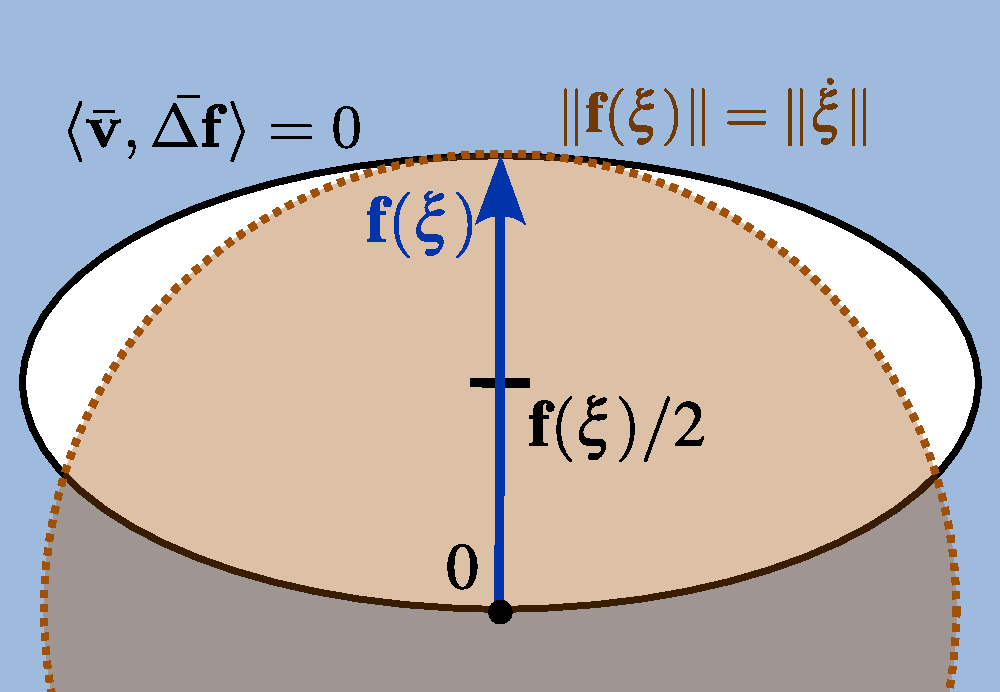
\includegraphics[width=\textwidth]{figures/passivity_analysis_wide}}
	  \caption{$\matd{S}_1^f > \matd{S}_2^f$, $w \approx 0$}
	  \label{fig:passivity_analysis_wide}
    \end{subfigure}\hfill%
    \begin{subfigure}{0.49\columnwidth}
    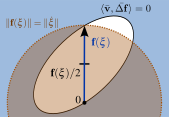
\includegraphics[width=\textwidth]{figures/passivity_analysis_skew}
	\caption{$\dotprod{\vect f(\vecs \xi)}{\vect q_1} \neq \| \vect f(\vecs \xi)\| \; \| \vect q_2\| $ }
      \label{fig:passivity_analysis_skew}
    \end{subfigure}
	\caption{
		The stability is ensured even if the controller can temporarily accelerate the system  to reach a velocity $\dot{\vecs \xi}$, which is faster than the desired velocity $\vect f(\vecs \xi)$ (white region).
		This happens when the eigenvalues of the damping matrix $\matd{D}(\vecs \xi)$ are not uniform (a) or the stretching vectors $\vect q_1$ and $\vect q_2$ are not orthogonal (b). 
	In both cases, the region of non-passivity is elliptical (black circle).
}
	\label{fig:passivity_analysis_varied}
\end{figure}
\fi


% Note, that in the case of $\langle e_2, e_n \rangle \neq 0$ the choice of $e_2$ does not matter as the corresponding  weight from \eqref{eq:eig2_weight} is $w_2 = 0$, hence it $\lambda_2 = \lambda$, as all eigenvalues.

% \section{Collision Avoidance} \label{sec:collision_avoidance}

% \subsection{Disturbance Repulsion}
The principal goal of the controller introduced in the previous section is its ability to ensure collision avoidance in the presence of external disturbances.
However, the control force $\vect \tau^c$ proposed in \eqref{eq:control_command} does not explicitly consider external forces. Yet, it is designed to correct the agent's velocity $\dot{\vecs \xi}$ if it deviates from the desired velocity $\ddot{\vecs \xi}$.\footnote{Note that for a discrete-time (digital) controller, this results in a delay.}

Since interaction with the environment results in a force on the system, often over a short period $\Delta t \ll 1$.  Hence, we can define the velocity after impact $\vect v^I$ as:
\begin{align}
	 % \begin{split}
	\vect v^I
	  \approx \int_{t^I}^{t^I + \Delta t} \ddot{\vecs \xi} dt  
	  \approx \int_{t^I}^{t^I + \Delta t} \matd{M}^{-1}(\vecs \xi)  \vecs \tau_e \, dt  
	 % \end{split}
	  \label{eq:impact_velocity}
\end{align}
using the controller from \eqref{eq:robot_dynamics}, and under absence of the control force $\vecs \tau_c$ during this short timeframe. Additionally, $\{\vect \xi \}_{t^I}$ is the velocity before the impact.
 
% Since the magnitude of the normal is limited to $1$, the control weight is limited as: 
% \begin{equation}
% w(\vecs \xi) \geq \frac{\Gamma^{\mathrm{crit}} - \Gamma(\vecs \xi)}{\Gamma^{\mathrm{crit}} - 1}
% \end{equation}
% under the assumption that $\Gamma^{\mathrm{crit}} \geq 1$.

% Using the controller design from \eqref{eq:control_command} the velocity can be computed as:
% \begin{equation}
% \begin{split}
% 	\{ \vecs{\dot \xi} \}_{t} 
% 	& = \int \vecs{\ddot \xi} \, dt = \int \matd{M}^{-1} \matd{D}  \bigl( \vecs{\dot \xi} - \vecs f(\vecs \xi) \bigr) \, dt \\
% 	& = \int \matd{M}^{-1} \matd{D} \bigl( \vecs{\dot \xi} - \vecs f(\vecs \xi) \bigr) \, dt \\
% 	& = \matd{M}^{-1} \int \left( (1 - w) \matd{D}^f + w \matd{D}^{o} \right)  \bigl( \dot{\vecs \xi} - \vecs f(\vecs \xi) \bigr) dt\\
% 	& = \matd{M}^{-1} \int  \matd{D}\bigl( \vecs \xi - t \vecs f(\vecs \xi) \bigr) + C_t \\
% 	% &  \underset{}\{ {\vecs \xi} \}_0 = \vecs f(\vecs \xi) + \vecs v^I{=} \matd{M}^{-1} \matd{D}  \left( \xi - t \vecs f(\vecs \xi) \right) + C_t \\
% 	&  = \matd{M}^{-1} \matd{D}  \bigl( \vecs \xi - \{\vecs \xi\}_0  - t \vecs f(\vecs \xi) \bigr) + \vecs f(\vecs \xi) + \vecs v^I \\
%     % & \approx \int \matd{M}^{-1} \matd{D} \vect f(\vecs \xi) \, dt
% \end{split}
% \label{eq:velocity_evolution}
% \end{equation}
% using $\{ {\vecs \xi} \}_0 = \vecs f(\vecs \xi) + \vecs v^I$ to find the integration constant $C_t$.

Furthermore, let us consider a desired velocity $\vect f(\vecs \xi)$, which is a constant, collision-free vector field parallel to the surface of a flat obstacle surface (see Fig.~\ref{fig:disturbance_with_parallel_velocity}):
\begin{equation}
	\dotprod{\vect f(\vecs \xi)}{\vecs n(\vecs \xi)} = 0
	 \qquad
\vect f(\vecs \xi) = \text{const.}
\, , \;
\vect n(\vecs \xi) = \text{const.}
\label{eq:parallel_velocity}
\end{equation}
where $\vecs n(\vecs \xi)$ is the surface's normal vector, and the agent moves in a straight line, hence we can neglect the Coriolis effect. For disturbances in such environments, we show that our approach can ensure the impenetrability of the obstacle up to an upper bound on the magnitude of the disturbance:

\begin{lemma} \label{lemma:damping_collision_avoidance}
	Consider a point-mass agent with mass $m \in \mathbb{R}_{>0}$, whose motion evolves according to the rigid body dynamics given in \eqref{eq:robot_dynamics} controlled by \eqref{eq:control_command}, with constant damping matrix $\matd{D}$ from \eqref{eq:damping_summation}. The agent tracks a constant reference velocity ${\mathrm{f}}$, whose vector field moves parallel to a flat obstacle as given in \eqref{eq:parallel_velocity}. Any motion path initiated in free space will remain collision-free for all times, i.e., $\Gamma( \{\vecs \xi_t\}) \geq 1$ with $t \geq 0$ if the impact velocity $v^I$ as given in \eqref{eq:impact_velocity} at time $t=0$ is limited by $\| \vect v^I\| < s^{\mathrm{f}} \| \vecs \xi - \vecs \xi^b \| / m$, with respect to the closest surface point $\vecs \xi^b \in \mathbb{R}^N$.
\end{lemma}

% \begin{lemma}
% 	A dynamical system evolves with the rigid body dynamics given in \eqref{eq:robot_dynamics} controlled by \eqref{eq:control_command}, with damping matrix $\matd{D}$ from \eqref{eq:damping_summation}, and a negligible Coriolis effect.
%     A point-like agent starting at position $\vect p = \{{\vecs \xi}\}_0$ close to the surface, i.e., $\Gamma( \vect p) \approx 1$ is guided by a velocity field $\vect f(\vecs \xi)$ parallel to the surface with a starting velocity $\vect v^0= \vect f(\{{\vecs \xi}\}_0)$.
%     A large disturbance towards the obstacle results in a velocity of $\{\dot{\vecs \xi}\}_0 = \vect v^I +  \vect v^0$ after the impact, with $\| \vect v^I \| \gg \| \vect v^0 \|$.
% 	A motion starting in free space remains collision-free for all times, i.e., $\Gamma( \{\vecs \xi_t\}) \geq 1$ with $t \geq 0$ if the impact velocity is limited by $\| \vect v^I\| < s^{\mathrm{o}} \| \vecs \xi - \vecs \xi^b \| / m^{\mathrm{min}}$, with respect to the closes surface point $\vecs \xi^b \in \mathbb{R}^N$ and mass $m \in \mathbb{R}_{>0}$.
% \end{lemma}

\begin{proof}
According to the Bony-Bezis theorem \parencite{bony1969principe}, the trajectories are collision-free if there is zero velocity towards the obstacle on the surface, i.e.,
\begin{equation}
	\left| \vect n(\vecs \xi)^T \, \{ \vecs{\dot \xi} \}_{t} \right| = 0 
	\quad \forall \, \Gamma(\vecs \xi) = 1
	\label{eq:bezis_theorem}
\end{equation}

We want to find the time when the agent stops moving towards the obstacle, enabling us to evaluate the distance traveled as a function of the velocity after disturbance $\vect v^I$. 
Let us assume without loss of generality that the disturbance occurs at time $t=0$. Hence, the velocity at time $T$ can be computed as:
\begin{equation}
\begin{split}
	\{ \vecs{\dot \xi} \}_{T} 
	& = \int_0^T \vecs{\ddot \xi} \, dt = \int_0^T \matd{M}^{-1} \matd{D} \left( \vecs{\dot \xi} - \vect f(\vecs \xi ) \right) \, dt \\
	& = \matd{M}^{-1} \int \left( (1 - w) \matd{D}^f + w \matd{D}^{o} \right) \left( \vecs{\dot \xi} - \vect f (\vecs \xi ) \right) dt \\
	\end{split}
\label{eq:velocity_evolution}
\end{equation}

Furthermore, since the vector field, $\vect f(\vecs \xi)$ is constant and the obstacle's surface does not have any curvature, it follows from \eqref{eq:damping_summation} that the damping matrices  $\matd{D}^o$ and $\matd{D}^f$ are constant.
Moreover, by design of the damping matrices, from \eqref{eq:first_obstacle_basis} it follow that $\matd{D}^o(\vecs \xi) \vect n(\vecs \xi) = s^o \vect n(\vecs \xi)$, and from  \eqref{eq:velocity_unit_vector} that $\matd{D}^f(\vecs \xi) \vect n(\vecs \xi) = s^f \vect n(\vecs \xi)$. 

From \eqref{eq:bezis_theorem} follows that it is sufficient to observe the normal component of the vectors only. Thus, in the rest of this paragraph, the components along the normal are denoted by scalar values, e.g. $\dot \xi = \dotprod{\dot{\vecs \xi}}{\vecs n(\vecs \xi)} \vecs n(\vecs \xi)$.
Hence, we get:
\begin{align}
	0 & = \left| \vect n(\vecs \xi)^T \, \{ \vecs{\dot \xi} \}_{t} \right| 
	  = \frac 1 m \int_0^T ( (1-w) \vect n^T \matd{D}^f \vect n + w s^{o} ) \, {\dot \xi} \, dt \nonumber \\
	   & < \frac 1 m \int_0^T  s^{f}  \, {\dot \xi} \, dt 
	   = \frac{s^f}{m} (\xi - \{ \xi \}_0 ) + v^I \, dt 
\end{align}
where $m = \max{\left(\text{eig}(\matd{M})\right)}$, with the maximum displacement as:
\begin{equation}
	\| \{\xi \}_0 - {\xi} \| \leq \| v^I \| {m} / {s^{\mathrm{f}}} 
\end{equation}
% To see when the differences reaches zero, we can compute
% \begin{equation}
%  \|	\{ \vecs{\dot \xi} \}_T - \vect f(\vecs \xi) \| = 0
%  \quad \Rightarrow \quad
%     \| \vecs{\xi}_1 -  \vect p_1 \| = \| \vecs v^I_1 \| {m} / {s^{\mathrm{o}}} 
%  \end{equation}
\end{proof}

Lemma~\ref{lemma:damping_collision_avoidance} assumes constant velocity field $\vect f(\vecs \xi)$ and flat obstacle surface. This is an appropriate assumption for large velocities after disturbances towards the obstacle, i.e., $\| \vect v^I \| \gg \| \vect f(\vecs \xi) \|$ and starting close to the surface. Since the distance traveled has to be flat to avoid collision, the vectorfield is likely to show small changes, and the surface has little deviation. 

\begin{figure}[htb]
\centering
 % \begin{subfigure}{0.99\columnwidth}
  \centerline{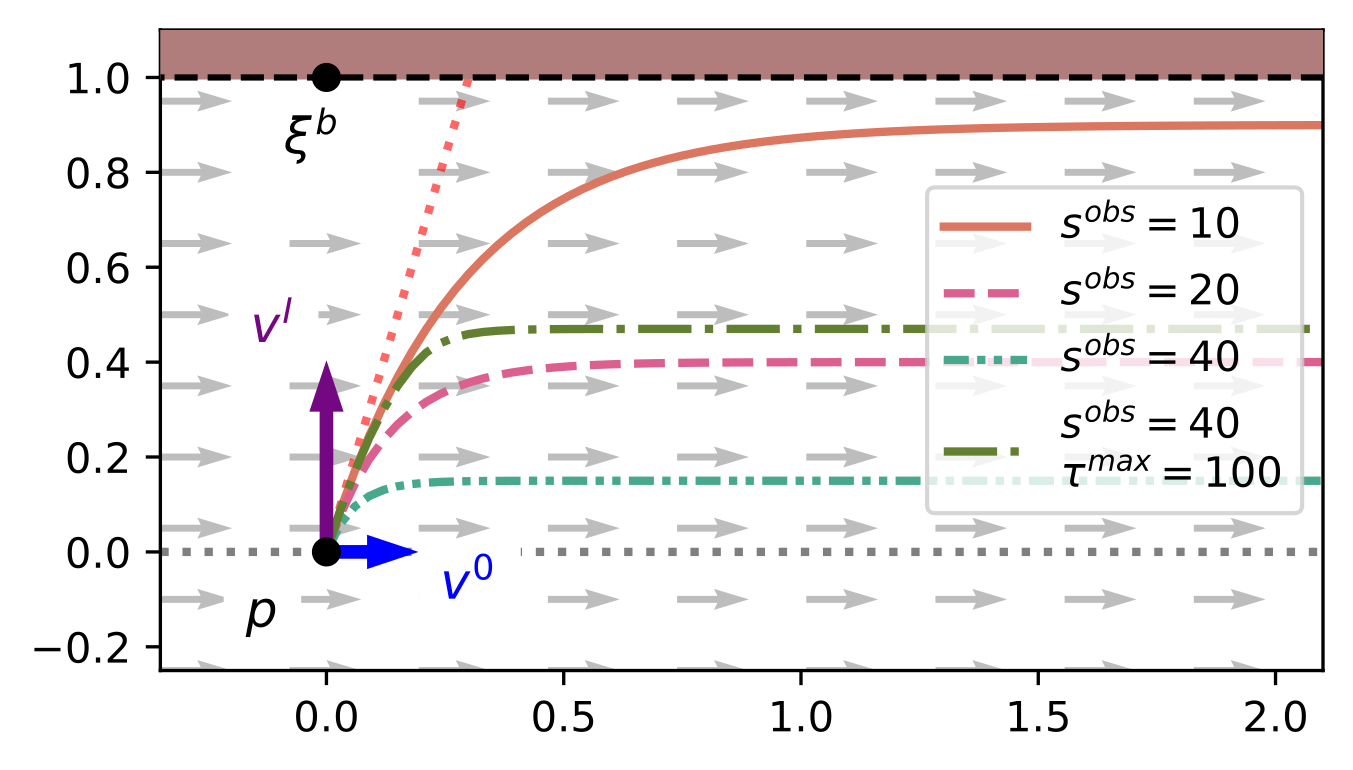
\includegraphics[width=0.99\columnwidth]{figures/parallel_avoidance_obstacle}}
  \caption{A disturbance occurs of a point-agent at position $\vect p^0$ with velocity after the impact of $\{ \dot{\vecs \xi} \}_0 = \vect v^0 + \vect v^I$. A high damping in the direction of the obstacle in the presence of a constant velocity field (gray) ensures collision avoidance. Whereas different damping values $s^{\mathrm{o}}$ and optionally a maximum repulsion force $\vecs \tau^{\mathrm{max}}$ lead to different trajectories.}
  \label{fig:disturbance_with_parallel_velocity}
% \end{subfigure}
\end{figure}
    
Nevertheless, there is no guarantee against drifting into obstacles in the presence of highly curved surfaces and velocity fields. \iflong This is further discussed during the experiments in Section~\ref{sec:position_noise}, where the increased damping towards the obstacle significantly reduces collision in such scenarios. \fi However, designing a repulsive field as proposed in \parencite{huber2023avoidance} can ensure collision avoidance in such scenarios.

\iflong
% \subsection{Disturbance Repulsion with Force Limit}
All robotic systems have a maximum force that they can exert on the environment based on the motors, geometry, and state, $\tau_c^{\mathrm{max}} \in \mathbb{R}_{>0}$. Such a limiting force decreases the impact velocity a controller can handle while ensuring collision avoidance, as shown in Fig.~\ref{fig:disturbance_with_parallel_velocity}. Nevertheless, a maximum control force can be interpreted as adapting damping; hence, the passivity from Theorem~\ref{theorem:passivity} holds.
\fi


\ifthesis
\section{Discrete Time Behavior} \label{sec:discrete_time_behavior}
\else
\subsection{Discrete Time Behavior} \label{sec:discrete_time_behavior}
\fi

So far, we've considered that the system is continuous time. 
This is a reasonable assumption, if we have a high sampling time $\Delta t$, compared to the dynamics, i.e., $\| \Delta t \, \dot{\vecs \xi} \| \ll 1$.
However, any digital controller sends a discrete control signal. To reject the disturbances in the presence of obstacles, a high control force is exerted (while remaining within the control robot's limits), hence $\| \Delta t \, \vecs \tau^c \| \gg 1$. 
In this case, it is crucial to analyze the discrete-time system to guarantee stability, as high damping can lead to unstable behavior, see Figure~\ref{fig:discrete_controller_parameters_comparison}).

\begin{figure}[htbp]
\centering
  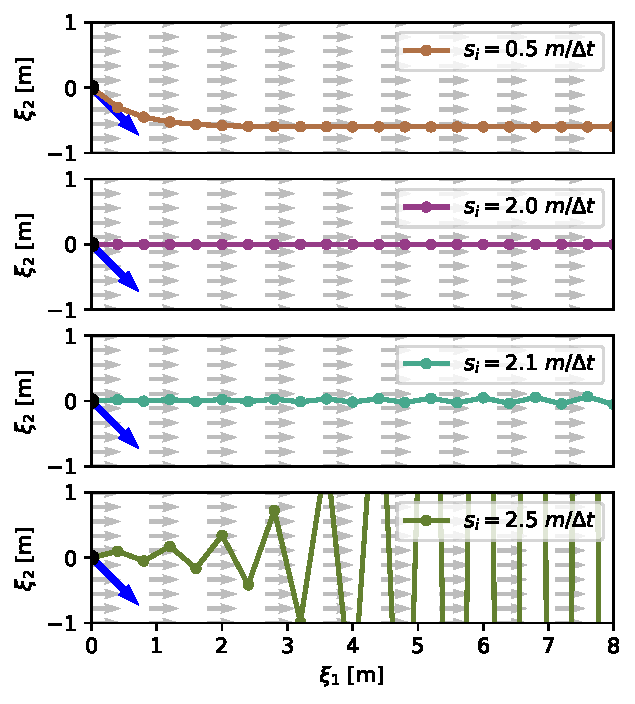
\includegraphics[width=\columnwidth]{figures/discrete_controller_parameters_comparison}
  \caption{An agent has the desired velocity $\vect f(\vecs \xi) = [1, 0]^T$ (gray arrow), and a control matrix $\matd{D}$ with damping values equal in all directions and the smallest eigenvalue of the inertia matrix $m$. 
 The agent is disturbed (purple arrow) position $\vecs \xi_0 = [0, 0]^T$ and has a velocity of  $\vecs \xi_1 = [1, 1]^T$ after the impact. \\
  High damping leads to unstable behavior with increasingly high oscillations. Conversely, the lowest value leads to more deviation from the initial straight line resulting from the higher impedance. The critical value of $s_i = 2.0 m / \Delta t$ results in stable behavior with immediate correction to the desired velocity.}
  \label{fig:discrete_controller_parameters_comparison}
\end{figure}

For the discrete-time system, the position and velocity of the agent evolve as follows:
\begin{equation}
	\begin{bmatrix}
	 \vecs \xi_{t+1} \\ \dot{\vecs \xi}_{t+1}
	\end{bmatrix}
	=
	\begin{bmatrix}
	 \vecs \xi_{t} \\ \dot{\vecs \xi}_{t}
	\end{bmatrix}
	+ 
	\Delta t 
	\begin{bmatrix}
		\dot{\vecs \xi}_{t} \\ \ddot{\vecs \xi}_t 
	\end{bmatrix}
	\label{eq:discrete_time_dynamics}
\end{equation}

\begin{lemma}
	Let us consider a discrete-time system with the state as given in Eq.~\eqref{eq:discrete_time_dynamics}, and is governed by the controller from Eq.~\eqref{eq:control_command} and damping matrix $\matd{D}$ defined in Eq.~\eqref{eq:damping_summation}.
	The system is BIBO (bounded-input, bounded-stable) with respect input the desired velocity $\vect f(\vecs \xi)$ the velocity, and as output the agent's velocity $\dot{\vecs \xi}$ such that $\lim_{t \rightarrow \infty} \| \dot{\vect \xi} \| < \infty$, if all damping values are limited as $s_{d} \leq 2 \min \left( \text{eig}\left(\matd{M}\right)  \right) / \Delta t$ with $d=1.. N$.
\end{lemma}

\begin{proof}
The evolution of the discrete-time feedback system is given as:
\begin{equation}
	\begin{split}
	& \begin{bmatrix}
	 \vecs \xi_{t+1} \\ \dot{\vecs \xi}_{t+1}
	\end{bmatrix}
	=
	\begin{bmatrix}
		\vect \xi_t + \Delta t  \; \dot{\vect \xi}_t \\ \
		\dot{\vecs \xi}_t + \Delta t \, \matd{M}^{-1} \left( \matd{D} \left( \vect f(\vecs \xi_t) - \dot{\vecs \xi}_t \right) - \matd{C} \right)
	\end{bmatrix} \\
	&  = %\approx
	\begin{bmatrix}
		\matr{I} & \matr{I} \Delta t \\
		\vect{0} & \matr{I} - \Delta t \matd{M}^{-1} \matd D 
	\end{bmatrix}
	\begin{bmatrix}
		\vect \xi_t \\ \dot{\vect \xi}_t
	\end{bmatrix}
	+ \begin{bmatrix}
		\vect{0} \\ 
		\Delta t \, \matd{M}^{-1} \matd{D} 
	\end{bmatrix}
	\hat{\vect f}(\vecs \xi_t) 
	% & \approx 
	% \begin{bmatrix}
	% 	1 & \Delta t \\
	% 	\Delta t \matd{M}^{-1} \matd D \frac{\partial \vect f}{\partial \vecs \xi} & 1 - \Delta t \matd{M}^{-1} \matd D 
	% \end{bmatrix}
	% \begin{bmatrix}
	% 	\vect \xi_t \\ \dot{\vect \xi}_t
	% \end{bmatrix}
	\label{eq:discrete_time_proof}
	\end{split}
\end{equation}
where $\hat{\vect f}(\vecs \xi_t) = \vect f(\vecs \xi_t) - \matd{D}^{-1} C$.  The dependency on the state $\vecs \xi$ of the matrices $\matd{M}$, $\matd{D}$, and $\matd{C}$ are omitted for brevity. $\matr{I} \in \mathbb{R}^{N \times N}$ denotes the identity matrix.
As we look at global stability, we look at the updated velocity $\hat{\vect f}(\vecs \xi_t) = \vect f(\vecs \xi_t) - \matd{D}^{-1} \matd{C}$. Since the Coriolis force is bounded, it follows that if the system is BIBO stable for $\hat{\vect f}(\vect \xi_t)$, then it is also BIBO stable for $\vect f(\vecs \xi_t)$ 

BIBO stability of a discrete-time system requires that all the eigenvalues of the feedback matrix are smaller or equal to one \parencite{friedland2012control}.
The eigenvalues of the above feedback system are given as:
\begin{equation}
	\vect \lambda_1 = \text{eig}(\matr{I}) \qquad \vect \lambda_2 = \text{eig} \left(\matr{I} - \Delta t \, \matd{M}^{-1} \matd{D} \right)
\end{equation}
where both $\vect \lambda_1 \in \mathbb{R}^N$ and $\vect \lambda_2 \in \mathbb{R}^N$ denote a vector containing $N$ eigenvalues.
All eigenvalues of $\vect \lambda_{1, i} = 1, \; i = 1...N$, and enable a stable system. 
The second set of eigenvalues $\vect \lambda_2$  depends on the passive control term. 
However, since $\matd{M}$ and $\matd{D}$ are both positive definite, the eigenvalues are positive:
\begin{equation}
	\matd{M} > 0 \; , \;\; \matd{D} > 0 
	\qquad \Rightarrow \qquad
	\vect \lambda_{2, i} > 0 \quad i = 1...N
\end{equation}

Hence, we only have to consider the upper limit, and the system is stable if the maximum eigenvalue is limited to:
\begin{equation}
	\max \left(\vect \lambda_2 \right) \leq 1 
	\quad \Rightarrow \quad
	s_{i} \leq 2 \min \Bigl( \text{eig}\bigl(\matd{M}\bigr)  \Bigr) / \Delta t
\end{equation}
\end{proof}

The stability guarantees provide BIBO stability, hence the boundedness of the output. 
Since the first eigenvalues equal one, there is no global asymptotic convergence. 
In fact, in the system from \eqref{eq:discrete_time_proof}, it can be observed that when the input dynamics are zero, i.e., $\vect f(\vecs \xi) = \vect 0$, the system immediately stops. But there is no convergence to a specific position.
However, in most cases, the desired system should only reach zero at the attractor position, and hence, we expect convergence to such a point.

\ifthesis
Yet, asymptotic stability is not guaranteed for general nonlinear input dynamics. Especially for dynamics with high curvature and low damping value, the final trajectory can end up in limit cycles ((Figure~\ref{fig:discrete_controller_parameters_comparison_stable}).
\fi

In practice, it is useful to use a large value for $s^{o}$ as it rejects disturbances towards the obstacles, and lower values for the dynamics following $s^{f}$ and damping in general direction $s^{c}$. Hence, we propose $s^{o} = 2.0 m / \Delta t$, $s^{f} = 1.0 / \Delta t$, and $s^c = 0.1 / \Delta t$.

\ifthesis

\begin{figure}[htbp]
\centering
  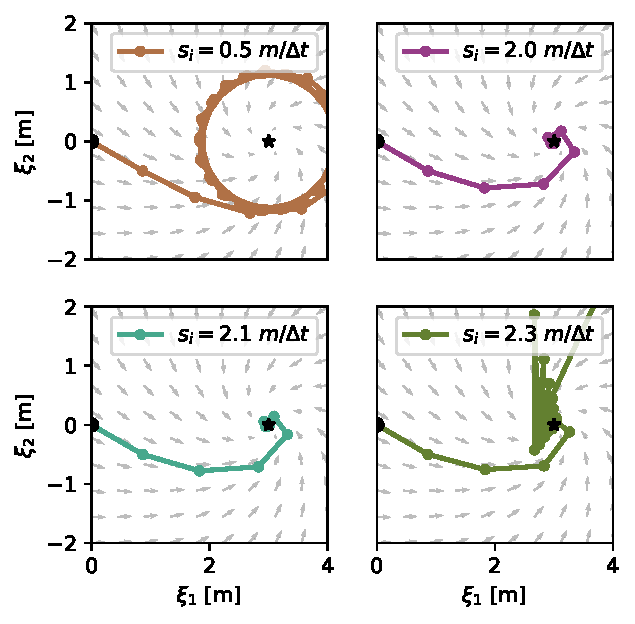
\includegraphics[width=\columnwidth]{figures/discrete_controller_parameters_comparison_stable}
\caption{An agent with the desired dynamics of
$\vect f(\vecs \xi) = \matr R(\pi / 6) (\vect \xi  - \vect \xi^a)$ where $\matr R(\cdot) \in \mathbb{R}^{N \times N}$ is the rotation matrix, and $m$ is the mass of the agent. We assume equal damping values $s_i$.
The controller with a critical stiffness of $2.0 m / \Delta t$ leads to fast convergence and a stable system. With lower damping (top left), there is a large drift of the system, which converges to a limit cycle. 
The high damping of $2.3 m / \Delta t$ leads to an unstable system. 
Interestingly, with damping of $2.1 m / \Delta t$ in combination with the nonlinear dynamics, we obtain a visibly stable system.}
  \label{fig:discrete_controller_parameters_comparison_stable}
\end{figure}

\fi

% continue here, noisy graphs ready to run

\section{Evaluation}  \label{sec:evaluation}

\subsection{Qualitative Comparison} \label{sec:qual_comp}
The control law presented was tested in simulation in Python. The state space is the Cartesian coordinates $xy$ in 2D and $xyz$ in 3D. In practice, the damping matrix $\matd D(\vecs\xi)$ and the control command $\vecs {\tau_c}$ are recomputed at each time step.\\

Let us compare traditional passive interaction control and the presented method (Fig.~\ref{fig_diff_obs_pass}). On the setup, the same disturbance is applied to both systems simultaneously. One can already see the robot equipped with traditional passive control (left) penetrates the obstacle, while ours (right) successfully damps the disturbance.

% \begin{figure}
% \centering
% \begin{subfigure}{0.8\columnwidth}
%   \centerline{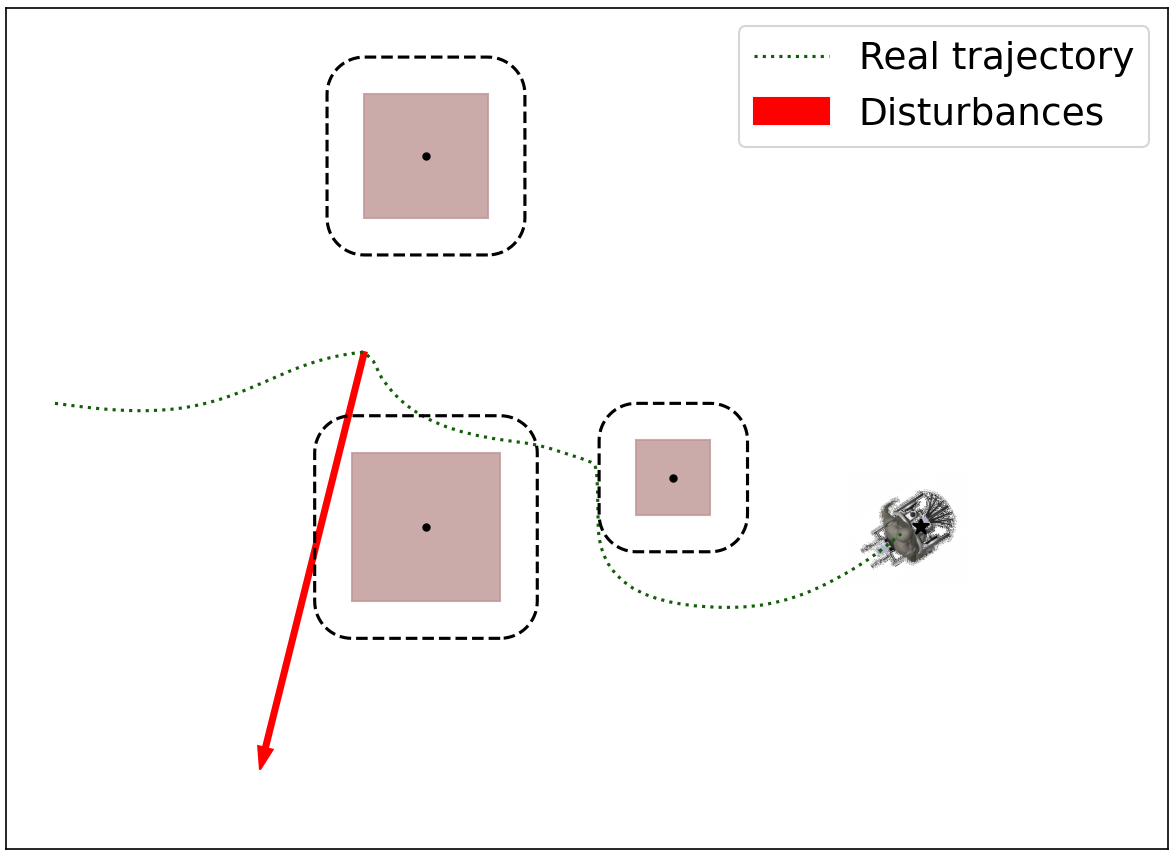
\includegraphics[width=\textwidth]{figures/run_without_pass.png}}
%   \caption{Traditional passive control}
% \end{subfigure}
% \begin{subfigure}{0.8\columnwidth}
%   \centerline{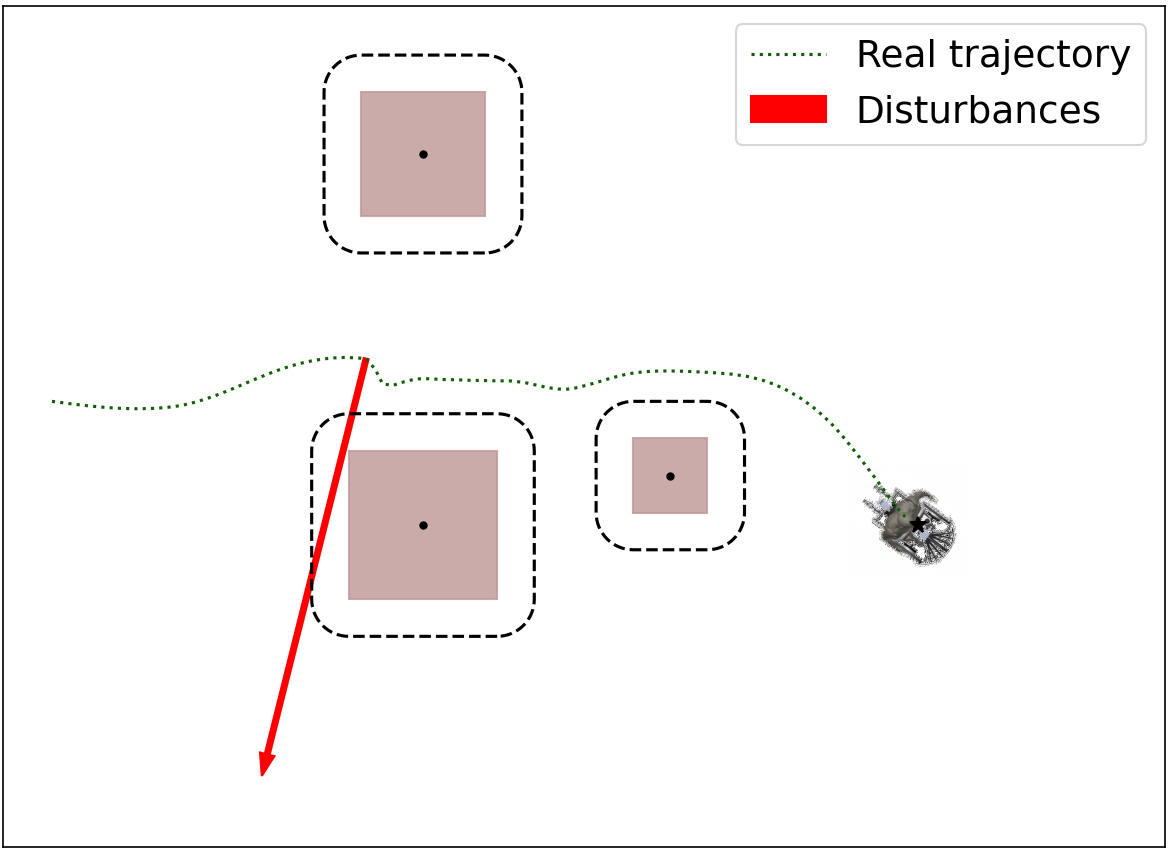
\includegraphics[width=\textwidth]{figures/run_with_pass.png}}
%   \caption{Obstacle aware passive control}
% \end{subfigure}
% \caption{Comparison of the two control methods}
% \label{fig:diff_obs_pass}
% \end{figure}

\begin{figure}
  \centering
  \centerline{\includesvg[width=0.95\columnwidth]{figures/multi_obstacle_with_damping.svg}}
  % \centerline{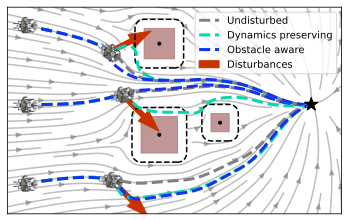
\includegraphics[width=0.5\textwidth]{figures/multi_obstacle_with_damping.svg}}
  \caption{The desired dynamics $\dot{\vecs \xi}$ in gray are as input for the force controller. 
  The mobile robot starting from the three positions, navigates safely to the attractor (black star) despite the disturbances (red arrows) when using the obstacle-aware controller.
  Conversely, the baseline (blue) leads to collision when the disturbance happens close to the robot.}
  \label{fig:obstacle_aware_damping_comparison}
\end{figure}

\subsection{Comparison to Reference Trajectory}
We will now look at the performance of our controller in different scenarios. Fig.~\ref{fig_run_with_obs} shows a simulation with 3 obstacles. The red arrows represent manually applied disturbances. The ideal trajectory is also displayed (perfect DS tracking, not subjected to real dynamics). Based on this simulation, we can observe the robots' behavior in different scenarios.

The first disturbance (A) pushed the robot in a direction perpendicular to the desired motion. Since we want compliance in this direction and the robot is far from any obstacle, it deviates greatly from its previous trajectory. It continues its path to the attractor on another DS line.

Another disturbance (B) pushed the robot toward the obstacle and was successfully damped, avoiding the collision.

A disturbance (C) pushed the robot away from an obstacle. The control algorithm is made such that when moving away from an obstacle, disturbances are not damped, and the robot shows compliant behavior. 

The last disturbance (D) was applied along the direction of motion. As the desired behavior is stiff in this direction, the robot almost kept the same speed and continued toward the attractor.

% \begin{figure}
% \centerline{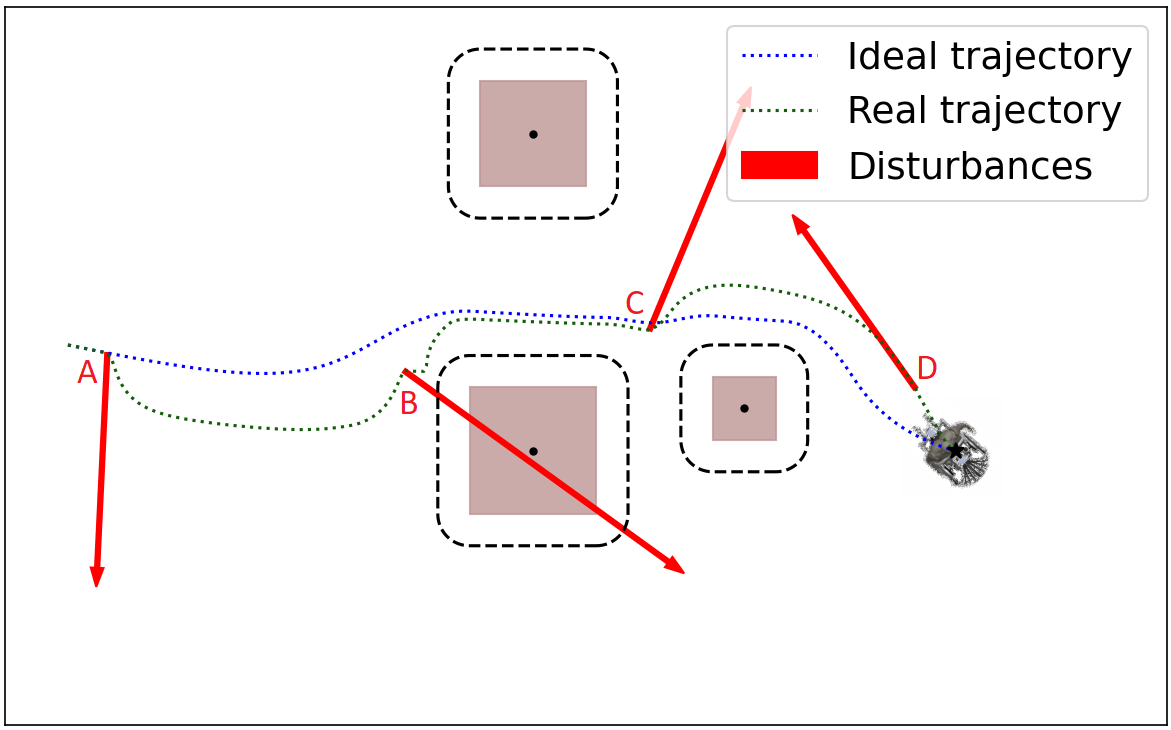
\includegraphics[width=0.5\textwidth]{figures/run_with_obs.png}}
% \caption{Simulation with a complex environment and disturbances applied to the robot}
% \label{fig_run_with_obs}
% \end{figure}

Furthermore, in Fig.~\ref{fig_run_damped_towards}, one can observe the feature described in Section~\ref{sec:damping_only_toward}, that only damps the disturbance towards the obstacle.
The first disturbance is highly damped, while the second is much less. This feature provides a natural behavior of moving away from obstacles, improving the margin of impenetrability. 

\subsection{Noise analysis}
Gaussian noise was added to the simulation to assert the control law's robustness. We added two types of noise, noise on the position measurements and noise on the velocity measurements. 

The experiment is done on a simple setup with one obstacle. The noise added has a mean of $0$, and the standard deviation is increasing linearly from $0.0$ to $0.7m$ for position and $0.0$ to $7.0 \frac{m}{s}$ for velocity measurements. For each noise level, the simulation was run 10 times. The output variable is the smallest distance of the agent from the obstacle during the simulation. This metric was chosen to observe how the noise could lead to a crash in the obstacle. 

For the noise acting on the position measurement, the controller presents good rejection for a small noise variance. As it increases, the robot's behavior quickly worsens (Fig.~\ref{fig_pos_noise}). The robot penetrates the obstacle for noises of standard deviation $ > 0.4 m$. An example of a run with $\sigma_{noise} = 0.7 m$ is shown in Fig.~\ref{fig_pos_noise_0_7}.

\begin{figure}
\centerline{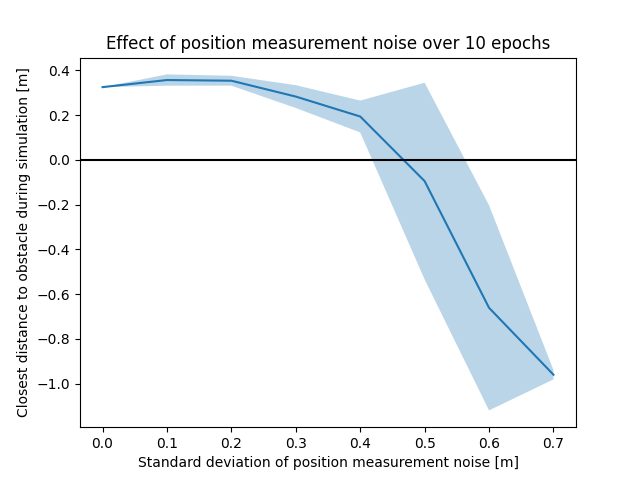
\includegraphics[width=0.5\textwidth]{figures/noise_pos_v2.png}}
\caption{Noise on the position measurements (shaded region are within one standard deviation from the mean)}
\label{fig_pos_noise}
\end{figure}

\begin{figure}
\centerline{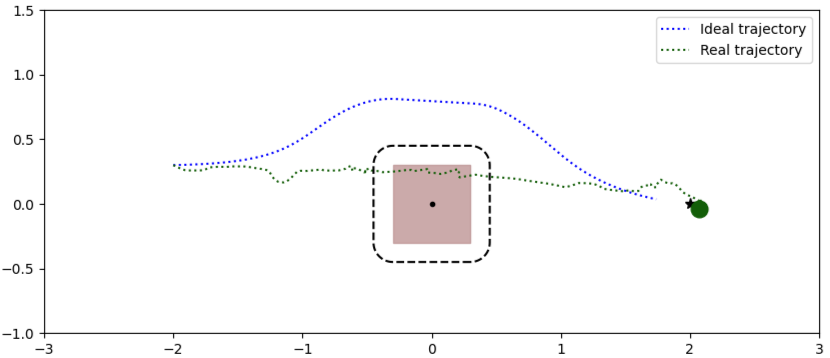
\includegraphics[width=0.5\textwidth]{figures/noise_effect_0_7.png}}
\caption{Noise on the position measurement with a standard deviation of 0.7 $m$ (with ideal trajectory displayed)}
\label{fig_pos_noise_0_7}
\end{figure}

The obstacle was never penetrated for the velocity measurement noise, asserting the robustness of the control for this type of noise (Fig.~\ref{fig_vel_noise}). Fig.~\ref{fig_2_vel_noise} provides an image of the simulation with big noise standard deviation ($4.0 \frac{m}{s}$). Thanks to the feature presented in Section~\ref{sec:damping_only_toward} (damping only toward the obstacle), the robot has even the tendency to drift away from the obstacle, increasing the safety margin.

\begin{figure}
\centerline{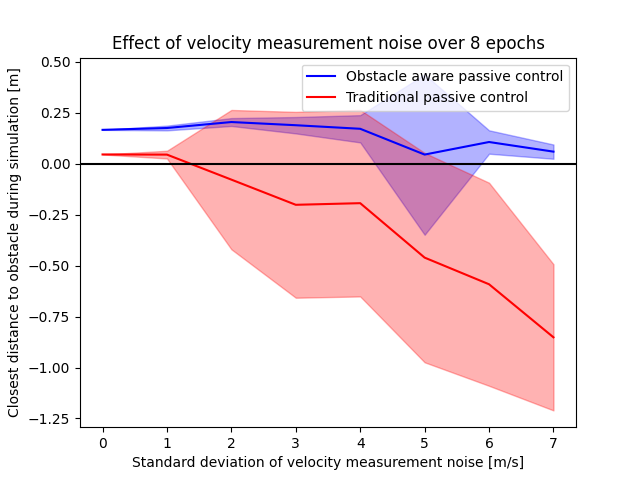
\includegraphics[width=0.5\textwidth]{figures/vel_noise_0.png}}
\caption{ NOT this one - Noise on the velocity measurements (shaded regions are within one standard deviation from the mean)}
\label{fig_vel_noise}
\end{figure}

\begin{figure}
\centerline{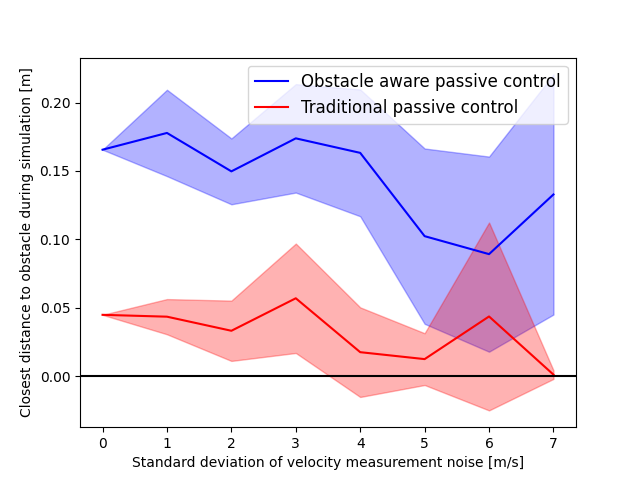
\includegraphics[width=0.5\textwidth]{figures/vel_noise_cliped_0.png}}
\caption{Noise on the velocity measurements (shaded regions are within one standard deviation from the mean) - NEW FINAL }
\label{fig_vel_noise}
\end{figure}

\begin{figure}
\centerline{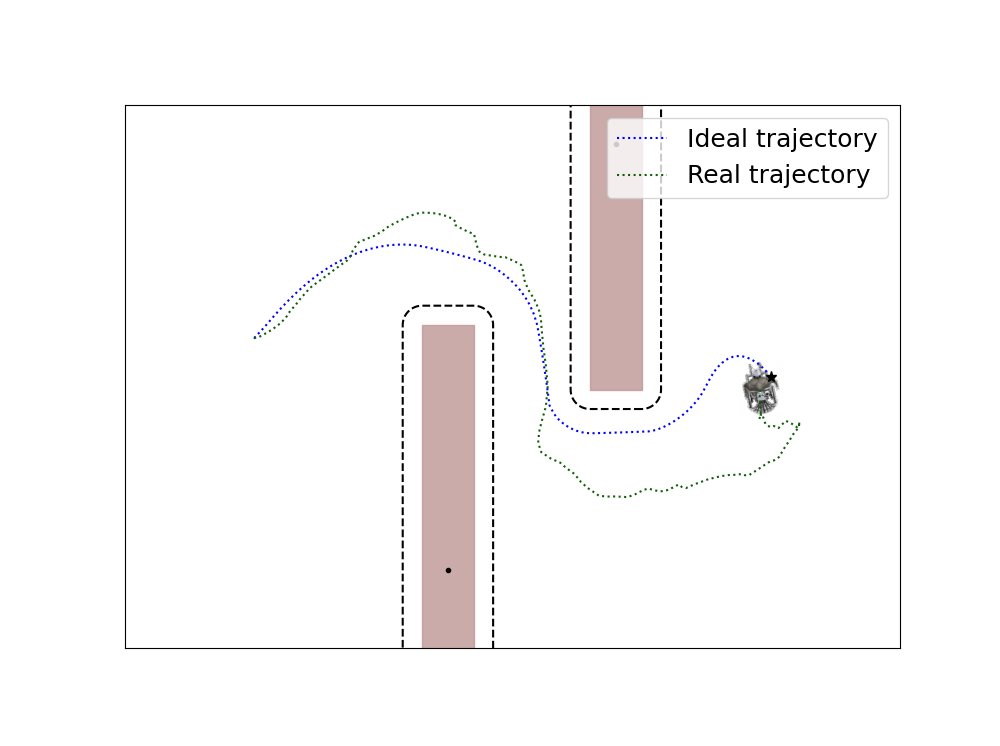
\includegraphics[width=0.5\textwidth]{figures/noise_setup.png}}
\caption{setup}
\label{fig_vel_noise}
\end{figure}


\begin{figure}
\centerline{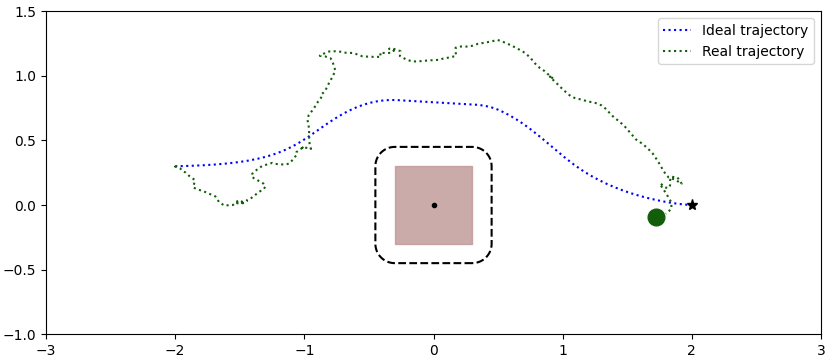
\includegraphics[width=\columnwidth]{figures/vel_noise_4.0.png}}
\caption{A simulation with noise on the velocity measurement with a standard deviation of $4.0 \frac{m}{s}$  (with ideal trajectory displayed)}
\label{fig_2_vel_noise}
\end{figure}


\subsection{Evaluation on Robot Arm}

\begin{figure}
    \centering
    \begin{subfigure}{\columnwidth}
      \centerline{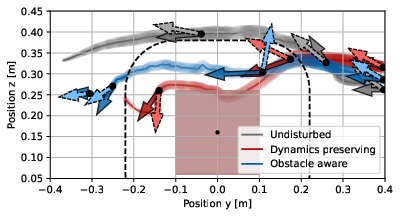
\includegraphics[width=\textwidth]{figures/robot_arm_trajectory_xyz}}
      \caption{Parallel to surface velocity}
      \label{fig:robot_arm_trajectory_xyz}
    \end{subfigure}
    \begin{subfigure}{\columnwidth}
    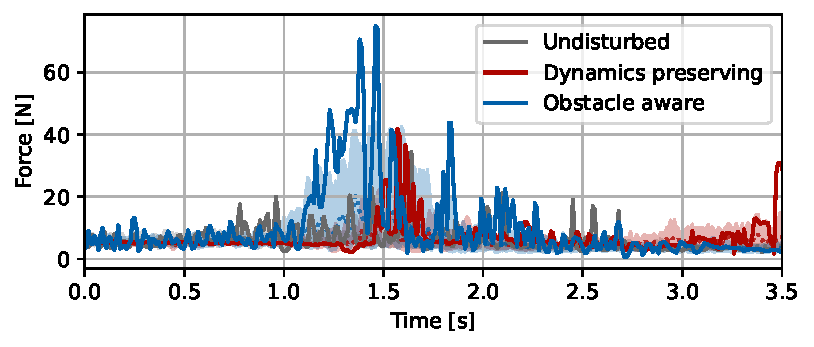
\includegraphics[width=\textwidth]{figures/trajectory_comparison_force_magnitude}
      \caption{Repulsive surface velocity}
      \label{fig:trajectory_comparison_force_magnitude}
    \end{subfigure}
    \begin{subfigure}{\columnwidth}
       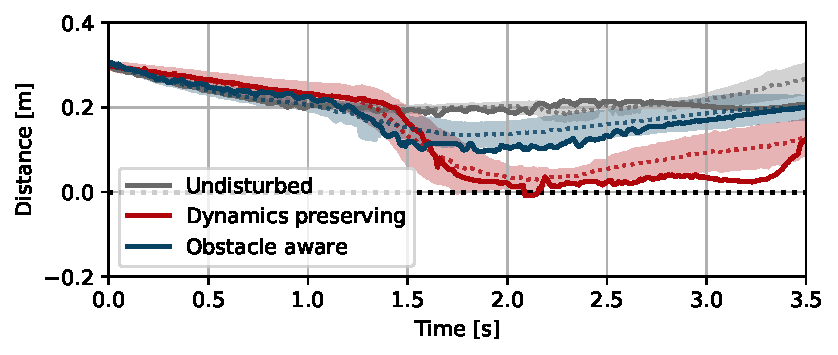
\includegraphics[width=\textwidth]{figures/robot_arm_trajectory_distance}
      \caption{Repulsive surface velocity}
      \label{fig:disturbance_with_repulsive_velocity}
    \end{subfigure}
    \caption{Comparison of the two control methods}
    \label{fig:evaluation_on_robot_arm}
\end{figure}

\section{Discussion}
Overall, the simulated robot shows pleasing results. It has good tracking performances, compliance in the direction perpendicular to the motion, and great damping of the disturbances towards obstacles.
Away from obstacles, the controller presented shows similar behavior as the one in \cite{kronander2015passive}. When approaching one obstacle, the control gets stiffer to avoid collisions without losing its tracking properties. This makes the proposed controller a suitable option to cumulate good tracking and safety regarding obstacle penetration.

\subsection{Applicability Approach}
Note, that the theoretical analysis from Theorem~\ref{theorem:passivity}, indicates passivity for any velocity-bounded, uniquely damped system. As a result, work such as the damping-based controller in  \cite{kronander2015passive} does not require an energy tank anymore.
Conversely, if the impedance controller has a proportional $\mathcal{K}$, the adaptive proportional term might induce instabilities even for stable desired dynamics as pointed out in \cite{ferraguti2013tank, kronander2016stability}.

% \renewcommand*{\bibfont}{\footnotesize}
% \printbibliography

